%%%%%%%%%%%%%%%%%%%%%%%%%%%%%%%%%%%%%%%%%%%%%%%%%%%%%%%%%%%%%%%%%%%%%%%%%%%%%%%%
%2345678901234567890123456789012345678901234567890123456789012345678901234567890
%    1     2     3     4     5     6     7     8

%\documentclass[letterpaper, 10 pt, conference]{ieeeconf} % Comment this line out if you need a4paper

\documentclass[a4paper, 10pt, conference]{ieeeconf}   % Use this line for a4 paper

\IEEEoverridecommandlockouts               % This command is only needed if 
                             % you want to use the \thanks command

\overrideIEEEmargins                   % Needed to meet printer requirements.

% See the \addtolength command later in the file to balance the column lengths
% on the last page of the document

% The following packages can be found on http:\\www.ctan.org
%\usepackage{graphics} % for pdf, bitmapped graphics files
%\usepackage{epsfig} % for postscript graphics files
%\usepackage{mathptmx} % assumes new font selection scheme installed
%\usepackage{times} % assumes new font selection scheme installed
%\usepackage{amsmath} % assumes amsmath package installed
%\usepackage{amssymb} % assumes amsmath package installed
\usepackage{graphicx, wrapfig, framed, lipsum}
\usepackage[font={small,it}]{caption}
\usepackage{subcaption}
\usepackage{amsfonts}
\usepackage{amsmath}
\usepackage{enumitem}
\usepackage{gensymb}
\usepackage{float}
\usepackage{hyperref}
\pagenumbering{roman}
\usepackage{pdflscape}
\usepackage{rotating}
\usepackage{color}
\usepackage{geometry}

\usepackage{xltxtra}
\setmainfont{Cambria}

\usepackage{filecontents}
\begin{filecontents*}{\jobname.bib}


@ARTICLE{Bioremediation, 
	author = { Bing Zhao and Chit Laa Poh}, 
	title  = {Insights into environmental bioremediation by microorganisms through functional genomics and proteomics}, 
	year  = {2008}, 
	journal = {Proteomics}, 
	volume = {8}, 
	number = {1}, 
	pages  = {874–881}
}
@ARTICLE{pseudomonas_putida, 
	author = {I.Rüegg and 
		T. Hafner and
		M. Bucheli-Witschel and
		T. Egli}, 
	title  = {Dynamics of Benzene and Toluene Degradation in Pseudomonas putida F1 in the Presence of the Alternative Substrate Succinate
	}, 
	year  = {2007}, 
	journal = {Eng. Life Sci}, 
	volume = {No. 4}, 
	number = {7}, 
	pages  = {331-342}
}
@ARTICLE{Pseudomonas_Veronii, 
	author = {Marian Morales and Vladimir Sentchilo and Claire Bertelli and Andrea Komljenovic and Nadezda Kryuchkova-Mostacci and Audrey Bourdilloud and Burkhard Linke and Alexander Goesmann and Keith Harshman and Francisca Segers and Fabien Delapierre and Damien Fiorucci and Mathieu Seppey and Evgeniya Trofimenco and Pauline Berra and Athimed El Taher and Chloé Loiseau and Dejan Roggero and Madeleine Sulfiotti and Angela Etienne and Gustavo Ruiz Buendia and Loïc Pillard and Angelique Escoriza and Roxane Moritz and Cedric Schneider and Esteban Alfonso and Fatma Ben Jeddou and Oliver Selmoni and Gregory Resch and Gilbert Greub and Olivier Emery and Manupriyam Dubey and Trestan Pillonel and Marc Robinson-Rechavi and Jan Roelof van der Meer}, 
	title  = {The Genome of the Toluene-Degrading Pseudomonas veronii Strain 1YdBTEX2 and Its Differential Gene Expression in Contaminated Sand.
	}, 
	year  = {2016}, 
	journal = {PLOS ONE}, 
	number = {DOI:10.1371/journal.pone.0165850}, 
	pages  = {1-21}
}

@online{toluene, 
	author = {Scottish Environment Protection Agency}, 
	title = {Pollutant fact sheet : Toluene}, 
	date  = {2017-11	}, 
	url  = {http://apps.sepa.org.uk/spripa/Pages/SubstanceInformation.aspx?pid=89}
}	

@ARTICLE{nodrawback, 
	author = {M.Cunliffe and M.A.Kertesz}, 
	title = {Effect of Sphingobium yanoikuyae B1 inoculation on bacterial community dynamics and polycyclic aromatic hydrocarbon degradation in aged and freshly PAH-contaminated soils}, 
	year  = {2006}, 
	journal = {Environmental Pollution}, 
	volume = {144}, 
	number = {1}, 
	pages  = {228-237}
}

@ARTICLE{bouchez, 
	author = {Bouchez and al.}, 
	title = {Ecological study of a bioaugmentation failure}, 
	year  = {2000}, 
	journal = {environmental biology}, 
	volume = {2}, 
	number = {2}, 
	pages  = {179-190}
}

@ARTICLE{oldarticle, 
	author = {R.M.Goldstein and L.M.Mallory and M.Alexander}, 
	title = {Reasons for possible failure of inoculation to enhance biodegradation.}, 
	year  = {1985}, 
	journal = {Applied and Environmental Biology}, 
	volume = {50}, 
	number = {4}, 
	pages  = {997-983}
}

@Manual{R,
	title = {R: A Language and Environment for Statistical Computing},
	author = {{R Core Team}},
	organization = {R Foundation for Statistical Computing},
	address = {Vienna, Austria},
	year = {2017},
	url = {https://www.R-project.org/},
}
\end{filecontents*}

\usepackage[
%backend=biber, 
natbib=true, 
style=numeric, 
sorting=none
]{biblatex}
\addbibresource{\jobname.bib}
\vspace{-2cm}
\title{\LARGE \bf
Can a toluene-degrading bacteria improve the growth of a bacterial community in case of toluene pollution?
}


\author{Léonard Jequier, Olivier Bützberger, Evan Bexkens and Victor Amstutz% 
}

\begin{document}

\newgeometry{left=1.7cm, right=1.7cm, bottom=2cm, top=2cm}
\vspace{-2cm}
\maketitle
\thispagestyle{plain}
\pagestyle{plain}
\pagenumbering{arabic}


%%%%%%%%%%%%%%%%%%%%%%%%%%%%%%%%%%%%%%%%%%%%%%%%%%%%%%%%%%%%%%%%%%%%%%%%%%%%%%%%

\begin{abstract}

In the case of an environmental pollution, the microbial community of the soil will have an important role in the degradation of the pollutant. However, adaptation to the sudden change in the soil composition is difficult for most bacterial communities. Bioaugmentation is a method that could be used to help them overcome the effect of pollution. It is the addition of bacteria able to degrade the pollutant into the contaminated environment. In our experiment, we chose to add \textit{Pseudomonas veronii} 1YdBTEX2 and \textit{Pseudomonas putida F1} (both tagged with fluorescent mCherry protein) to a bacterial community extracted from sand and to grow them either with toluene only or with mixed carbon\footnote{Mixed Carbon media composition : L-Arginine, D-Xylose, Aspartic acid potassium salt, 2-Hydroxybenzoic acid, L-Phenylalanine, L-Serine, Gamma Hydroxy butyric acid, D-cellobiose, alpha-D-Lactose, Putrescine, Itaconic acid, alpha-D-Glucose-1-phosphate, D-Glucosaminic acid, N-acetyl-D-glucosamine, 4-Hydroxy benzoic acid, D-Mannitol, meso-erytritol, Galacturonic acid, Methyl pyruvate, Tween 20. Each component in equal concentration} substrate. As the two \textit{Pseudomonas} strains we added are able to degrade toluene, we wanted to know if the addition of one of these strain to this bacterial community would have an effect on the growth of this community.
Our results are encouraging and would deserve some further experimentations. However, unlike usual bioaugmentation experiments in literature, our results indicate that the Sand Community was almost entirely replaced by \textit{Pseudomonas veronii} or \textit{Pseudomonas putida}.

%However, in the experiment conditions, the final amount of \textit{Pseudomonas} cells was way higher than the Sand Community cells, which means that the overall community was quite different from the starting Sand Community.

\end{abstract}


%%%%%%%%%%%%%%%%%%%%%%%%%%%%%%%%%%%%%%%%%%%%%%%%%%%%%%%%%%%%%%%%%%%%%%%%%%%%%%%%
\section{Introduction}
%alternative beginning

%Every surface, soil or liquid in our environment is colonised by multiple microorganisms, interacting with each other and forming communities. However, the whole complexity of the interactions are still today not always fully understood.
%One of the most important part of these communities is that they not only interact with one another but are able to interact with other organisms. These communities can be perturbed by the effects of pollution as spillage of oil or solvent. We decided to 

Every surface, soil or liquid in our environment is colonized by multiple microorganisms, interacting with each other and forming communities. However, the whole complexity of the interactions still isn't fully understood today.
In addition, these communities also interact with other organisms and can be perturbed by the effects of pollution such as oil or solvent spillage. We decided to use toluene as a pollutant for this experiment.

Toluene is an organic solvent widely used in the paint or cosmetic industry nowadays. It is a monoaromatic volatile molecule which is toxic and ecotoxic \cite{toluene}. 
When such event happens, one way to treat it is the use of bioremediation. There are several different techniques of bioremediation but they all have the same purpose: to use live organisms to get rid of pollutants. The technique that interested us in this experiment was bioaugmentation, the addition of a microorganism able to degrade the targeted pollutant to a native community, allowing it to grow back \cite{Bioremediation}.

The microorganisms we chose for our experiment were \textit{Pseudomonas putida} F1 (PP) and \textit{Pseudomonas veronii} 1YdBTEX2 (PV), both able to metabolize toluene \cite{pseudomonas_putida} \cite{Pseudomonas_Veronii}. The bacterial community on which we tested this procedure was extracted from sand (sand community (SC) collected at St-Sulpice beach, Switzerland).

To measure the number of cells in our culture we used flow cytometry\footnote{Flow cytometer, Novocyte : https://www.aceabio.com/products/nov\linebreak[0]ocyte-flow-cytometer/, Nov. 2017}. This technique consists of passing cells one by one through a capillary and hit each cell with a laser. It also allows us to differentiate cells by their fluorescent markers.

%ALTERNATIVE 1

%In our experiment we wanted to know if this ability to metabolize toluene could not only have a positive effect on a native community, for example by lowering the toluene concentration or by producing metabolites that the bacteria from SC could use as carbon source. Our hypothesis for this experiment was that the addition of \textit{Pseudomonas putida} or \textit{Pseudomonas veronii} will have an effect on SC growth, especially in a toluene-only media. 
%ALTERNATIVE 2 

%Our hypothesis for this experiment was that the addition of Pseudomonas putida or Pseudomonas veronii will have an effect on SC growth, especially in a toluene-only media.
%Ideed, we think that these Pseudomonas bacteria could produce metabolites the SC bacteria could use as carbon source or reduce the toluene concentration and thus it's toxic effect. This would lead to a better growth of the sand community in presence of one of these pseudomonas strains.

Our hypothesis for this experiment were that the addition of PP or PV will have an effect on SC growth, especially in a toluene-only media, because we think that these strains might produce metabolites the SC could use as carbon source or reduce the toluene concentration and thus its toxic effect. This would lead to a better growth of SC in presence of either PP or PV.


\section{Materials and methods}

\subsection{Experimental design}
Apart from SC, we used two bacterial strains : \textit{Pseudomonas veronii} 1YdBTEX2 (tagged with mCherry) and \textit{Pseudomonas putida F1}(also tagged with mCherry).

However, keep in mind that SC isn't a single species of bacteria, but rather a community containing potentially many different species.
%There were 3 bacterial cultures used for this experiment: \textit{Pseudomonas veronii} 1YdBTEX2 (tagged with mCherry, called PV), \textit{Pseudomonas putida F1}(tagged with mCherry, called PP) and a Sand Community, extracted from the beach of St-Sulpice. 
We experimented with two media: a mixed carbon medium\textsuperscript{1} and a Minimal Media 1x (MM) with only toluene as carbon source.


We separated the work into two weeks, testing SC and PP during Week 1 and SC and PV during Week 2. In each experiment, we tested the 2 communities and their interaction in mixed carbon and toluene.

\begin{figure}[H]

	  
		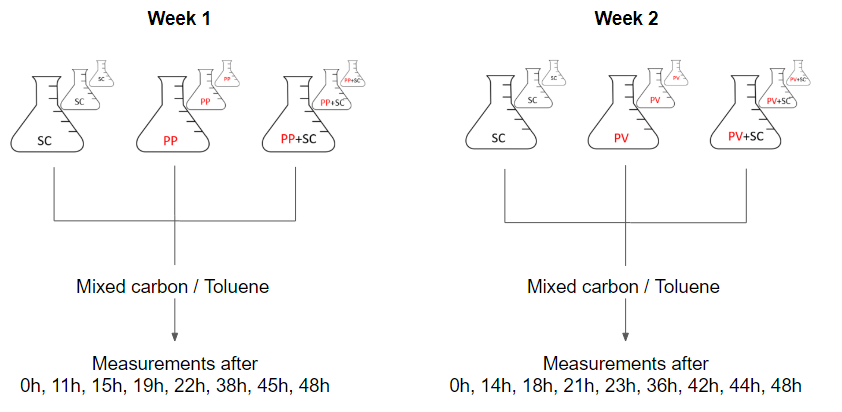
\includegraphics[width=9cm]{erlenmeyer.PNG}
		\caption{Experimental design. Experiments were separated into 2 weeks, with triplicates for each bacterial culture. The number of cells was measured at multiple timepoints.}
		\label{design_weeks}
	
\end{figure}

As controls, we used SC alone in both media, to prove that the medium has an effect and compare with the interaction of species. PP(or PV) alone in both media are used to show that the medium has no effect.
We therefore had 6 unique treatments, and used 3 replicates for each. We ended up with 18 cultures per experiment. These cultures were then sampled and counted regularly with a flow cytometer at different timepoints. The timespan between two timepoints had to vary to fit our personal schedules.


\subsection{Extraction of Sand Community (SC)}
The sand came from St-Sulpice. We took 200g of it and mixed it with 400 mL of 1x Minimal Media (MM) in a flask. We shaked it at 25°C, 115rpm for one hour, the time needed to extract the cells from the sand. The supernatant was collected in 50 mL falcon tubes, then centrifuged at 800rpm for 10 minutes. All the supernatant was then sieved through a 40 µm filter, and centrifuged at 4’000rpm for 30 minutes. The supernatant was discarded and the pellets re-suspended in 5 mL 1x MM. Then centrifuged at 800rpm for 10 minutes. We collected the supernatant and repeated this step until there was no visible pellet.



\subsection{Pseudomonas veronii and Pseudomonas putida}
The laboratory's samples were kept at -80°C, taken out at room temperature and streaked on LB plates with antibiotics (Gentamicin GM10). Incubated at 30°C, then one colony was streaked on MM 1x plates without added carbon. All the plates were put in a closed chamber containing 200 µL 100\% toluene. The plates were incubated at 30°C. Then took one colony, put it in liquid MM with 5 mM succinate, and incubated it at 30°C.

\subsection{Inoculation}
We put 20 mL of mixed carbon media [0.1mM] in nine flasks, and 20 mL of MM 1x in the other nine, where we added 200 µL toluene  50\% (100 µL toluene and 100 µL 2,2,4,4,6,8,8-Heptamethylnonane (HMN)\footnote{Oil used with volatile solvent to decrease their toxicity by slowing its release in the medium. Ref. https://www.sigmaaldrich.com/catalog/product/aldrich/128511?lang\linebreak[0]=fr\&region=CH, Dec. 2017}) in a tip sealed at the bottom. Toluene being volatile, it will then evaporate and dissolve in the liquid media. It will be the only source of carbon. We quantified the cells using flow cytometry, and calculated to put $10^{6}$ cells/mL in PV/PP alone flasks, SC flasks, and added twice $10^{6}$ cells in PPSC and PVSC flasks. The flasks containing toluene were sealed to avoid toluene leaks (Fig. \ref{flasks}).
They were incubated at 25°C and constantly shaken at 110rpm during 48 hours.

\subsection{Sampling and count of cells}
Every few hours (see Fig. \ref{design_weeks} for precise times), we took 3 samples from each flask to make technical replicates, and stained them with 4 µL SYTO-9 (50 µM), a  green fluorescent nucleic acid stain\footnote{ref. https://www.thermofisher.com/order/catalog/product/S34854, Nov. 2017}.  We then added 200 µL of each sample to the wells of a 96-well plate.

To measure the growth of our cells we used a flow cytometer. 
Since \textit{Pseudomonas putida F1} and \textit{Pseudomonas veronii} 1YdBTEX2 were tagged with mCherry (a red fluorescent protein encoded by mCherry gene, inserted downstream of the constitutive promoter of PP strain), and all the cells (both Gram positive and Gram negative cells) were stained with SYTO-9, we could differentiate PP/PV from SC. 
%\begin{figure} 
%	\centering
%	 \raggedright
%	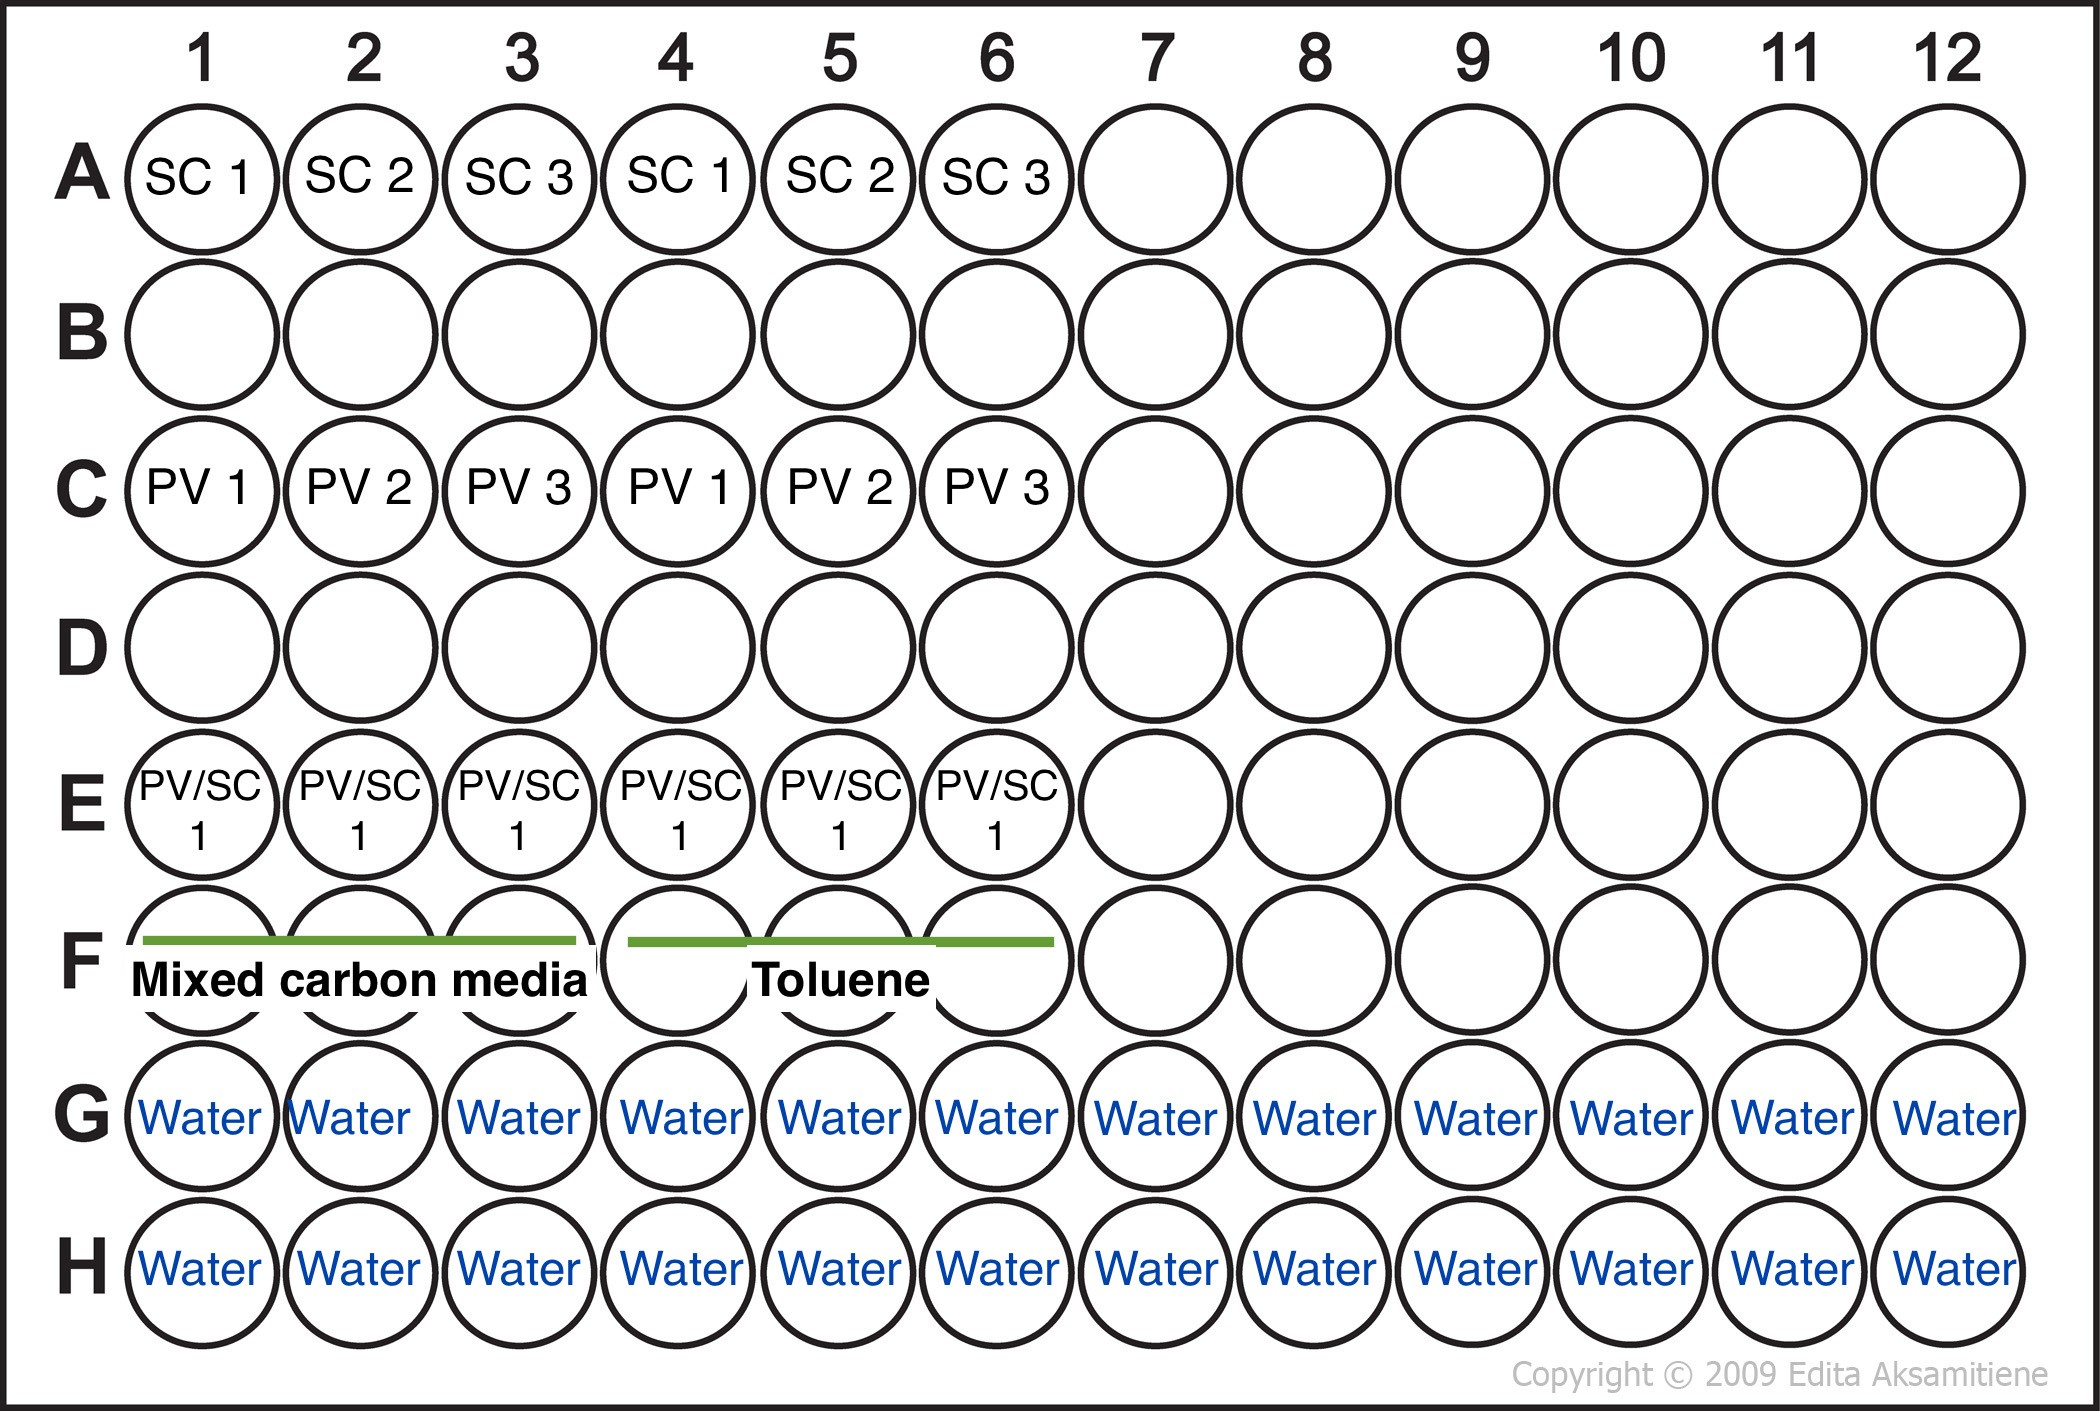
\includegraphics[width=8cm]{96wellplate.jpg}
%	\caption{96 well plate map used in our experiments. The numbers (1, 2, 3) represent the replicates\textsuperscript{*}.}
%	\small\textsuperscript{*} http://www.cellsignet.com/media/plates/96.jpg, Nov. 2017
%	\label{96wellplate}
%  
%\vspace{-0.5cm}	
%\end{figure}

\begin{figure}
		\hspace{-0.3cm}
		\begin{subfigure}{.25\textwidth}
			\centering			
			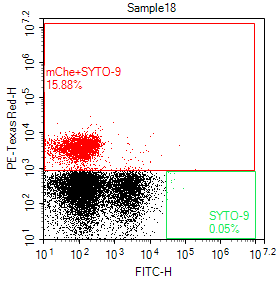
\includegraphics[width=4.3cm]{t8_unstained_ppsc1.png}
			\caption{}
			\label{scatter1}			
		\end{subfigure}%
		\begin{subfigure}{.22\textwidth}		
			\centering			
			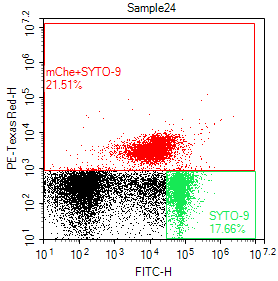
\includegraphics[width=4.3cm]{t8_stained_ppsc1.png}
			\caption{}
			\label{scatter2}			
		\end{subfigure}
		\caption*{Fig. \ref{scatter1}: Data of unstained sample (unstained PPSC in toluene, replicate 1, timepoint 8). \\ Fig. \ref{scatter2}: Data of stained sample (stained PPSC in toluene, replicate 1, timepoint 8). Horizontal axis : intensity of red fluorescence. Vertical axis : intensity of green fluorescence.}
		\label{scatterplot}
		\vspace{-0.5cm}
\end{figure}

The Fig. \ref{scatter1} and \ref{scatter2} are scatterplots of unstained (Fig. \ref{scatter1}) and stained (Fig. \ref{scatter2}) samples. The vertical axis shows the intensity of green fluorescence, while the horizontal axis shows the intensity of red fluorescence. 



On Fig. \ref{scatter1} a big black cluster and a red one above it can be observed. The black cluster is composed of SC cells and remaining particles. They show  low red and green fluorescence values. The PP cells express mCherry and therefore show strong red fluorescence, which causes an upwards shift on the plot, forming the red cluster above.

On Fig. \ref{scatter2} is a scatterplot of a sample from the same culture at the same timepoint but stained with SYTO-9. The SYTO-9 binds DNA and stains all the cells (PP alike) with a green fluorescence, which causes them to shift to the right side. However, the red fluorescence value still allows for a distinction between PP/PV and SC. The various residual particles (black cluster) are not affected by the SYTO-9. 

From the unstained sample, we were able to determine gates (the red and green frames on the scatterplots) to differentiate what we will consider as SC, PP/PV or simply residual sand particles. These gates could then be applied to each sample.

Also, we had to dilute our samples when the concentration of cell became too high. Otherwise we risked to clog the capillaries.
In the first week, we diluted our sample 10 fold at timepoint 1 and 100 fold from timepoint 2. In the second week, we diluted our sample 10 fold at timepoints 1 to 4 and 100 fold from timepoint 5.
We then adjusted the results to the original concentration during the analysis. 
%We can see on Fig. \ref{scatterplot} that the \textit{Pseudomonas} cells form a distinct, compact cluster (in red). The limitation between SC (in green) and remaining particles (in black) however, is a bit more subtle to determine. During the second week, we used an unstained measurement to determine a threshold of green fluorescence value from which we consider the particles to be cells (reminder: as SYTO-9 binds DNA and will stain only cells). We applied these gates to every sample of both weeks.


\subsection{Statistical method}
Finally, our data was composed of red and green fluorescent cell counts for each treatment, at 4 timepoints every day for two days. We used the R environment for all the analysis \cite{R}.\\
We represented graphically the logarithm of these counts over time for each replica and calculated the area under the curve. It allowed to summarize the data to one value per replica of each treatment (Fig. \ref{aucscw1}, \ref{aucppw1}, \ref{aucscw2}, \ref{aucpvw2}).
We performed four two-way crossed Anova to test the difference in growth of each Species separately between the substrate. For example, to test the difference in growth of SC in the first week, we used: \\
Explicative variables:
\begin{itemize}
	\item Species in culture: SC or SC + PP
	\item Media: Toluene or mixed carbon
\end{itemize}
Response variable:
\begin{itemize}
	\item Log of the area under the curve
\end{itemize}

\section{Results}
\subsection{Week 1 $\textendash$ SC, PP, PPSC}
\subsubsection{Total cell count comparison}


First, we are interested in the total cell count of each treatment. We look at the sum of both fluorescence counts.
In mixed carbon (Fig. \ref{totcountmixC1text}), PP and PPSC curves look very similar. SC seems to grow slower but catch up with the other culture after 40 hours.
In toluene (Fig. \ref{totcounttol1text}), PP and PPSC look again very similar. This time however, 
we don’t observe any growth in the SC culture.
This experiment shows no signs that growing PP and SC together influences the growth of the overall population or the total cell count after 48 hours, in a mixed carbon or toluene media (compared to the PP alone control).
Since the species are marked with different fluorescence, we can also compare the growth of each population separately in each treatment.\newline

%\begin{figure}[H]
%	\centering
%	
%	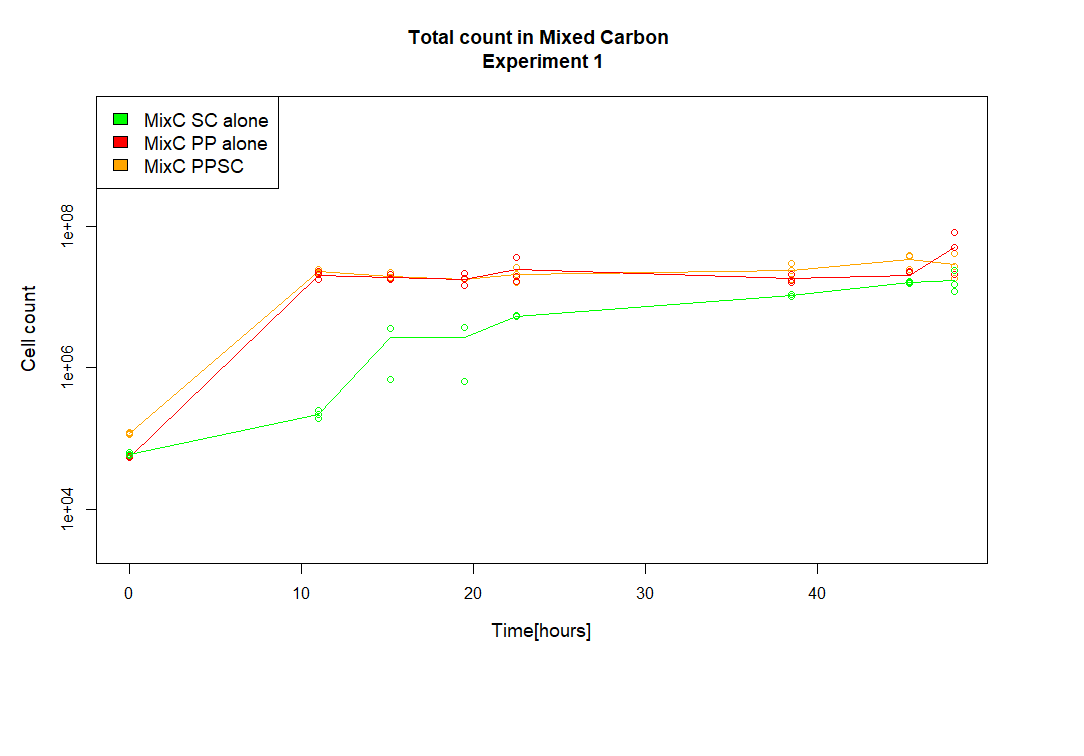
\includegraphics[width=9.3cm]{totcount_mixC1.PNG}
%	\caption{ADD CAPTION}
%	\label{totcountmixC1text}
%\end{figure}
%\begin{figure}[H]
%	\centering
%	
%	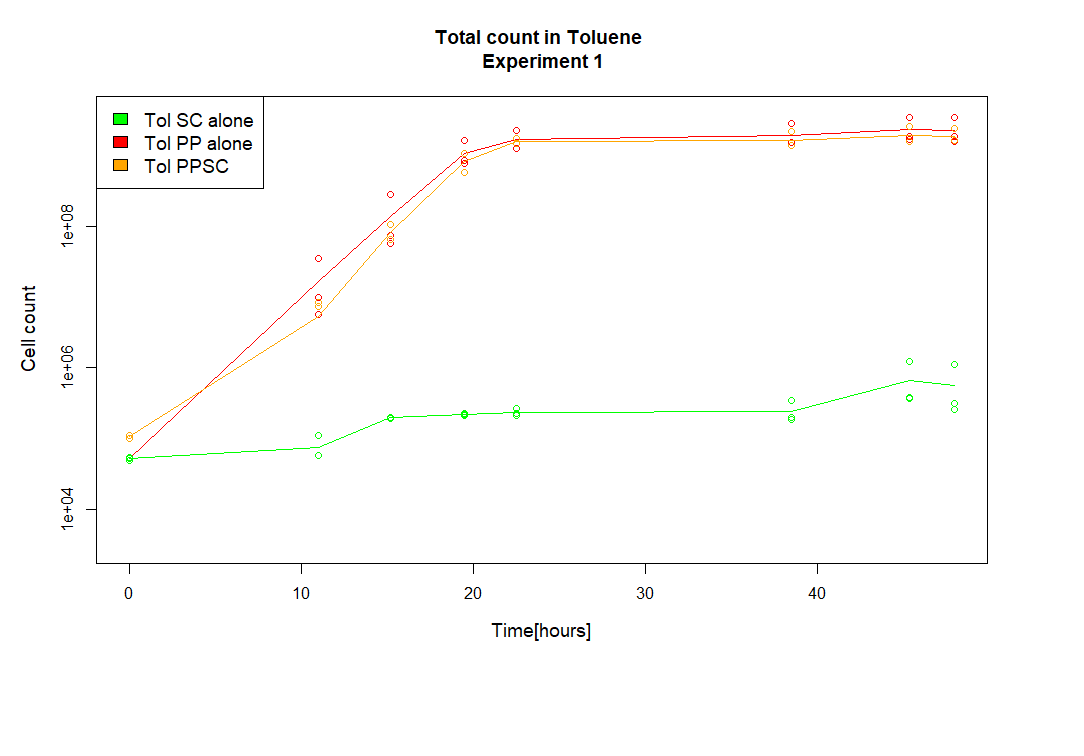
\includegraphics[width=9.3cm]{totcount_tol1.PNG}
%	\caption{ADD CAPTION}
%	\label{totcounttol1text}
%\end{figure}
%\begin{figure}[H]
%	
%	\begin{subfigure}{.5\textwidth}
%		\centering
%		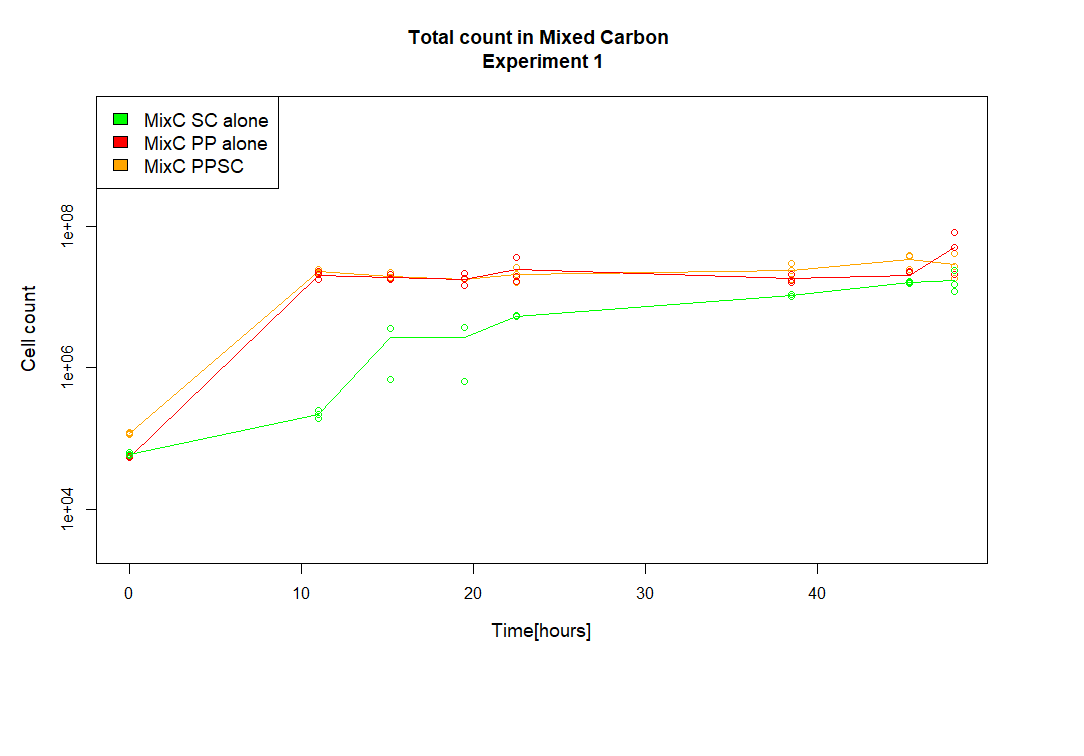
\includegraphics[width=9cm]{totcount_mixC1.PNG}
%		\caption{}
%		\label{totcountmixC1text}
%	\end{subfigure}
%	\begin{subfigure}{.5\textwidth}
%		\centering
%		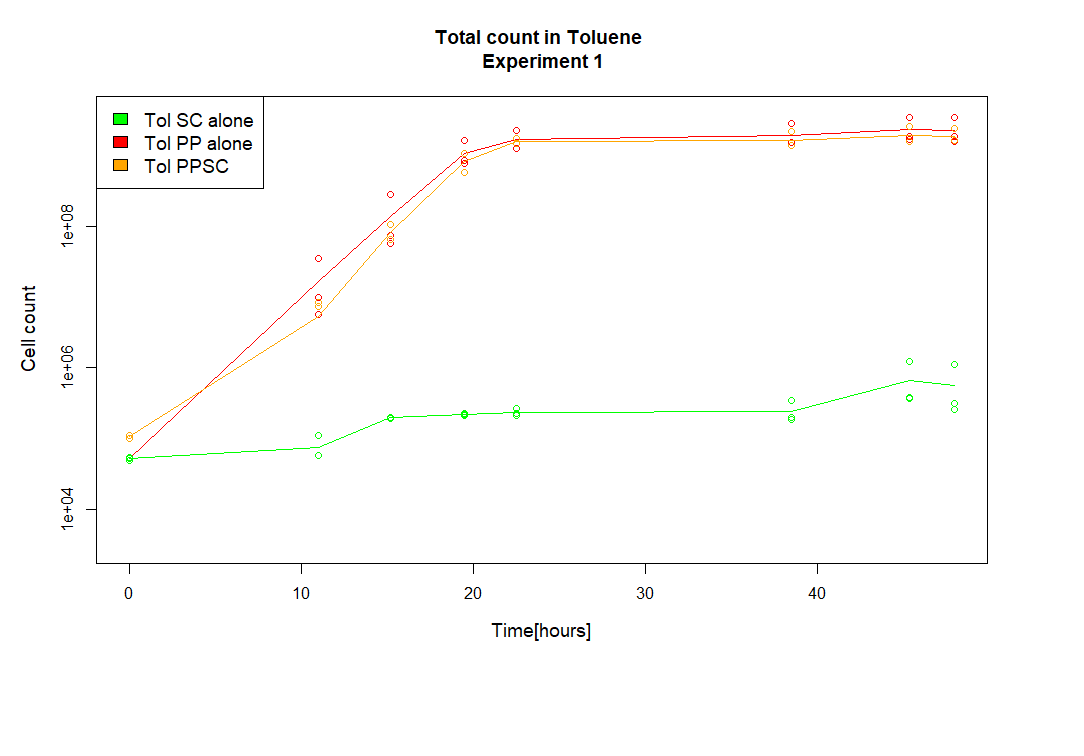
\includegraphics[width=9cm]{totcount_tol1.PNG}
%		\caption{}
%		\label{totcounttol1text}
%	\end{subfigure}
%	\caption{Fig. \ref{totcountmixC1text}: Total count (SYTO-9 Count + mCherry count) of SC, PP and PPSC over time in a mixed carbon medium during the first week. Fig. \ref{totcounttol1text} : Total count (SYTO-9 count + mCherry count) of SC, PP and PPSC over time in a toluene only medium during the first week.}
%	\label{totcount1}
%\end{figure}

\begin{figure}
	\centering
	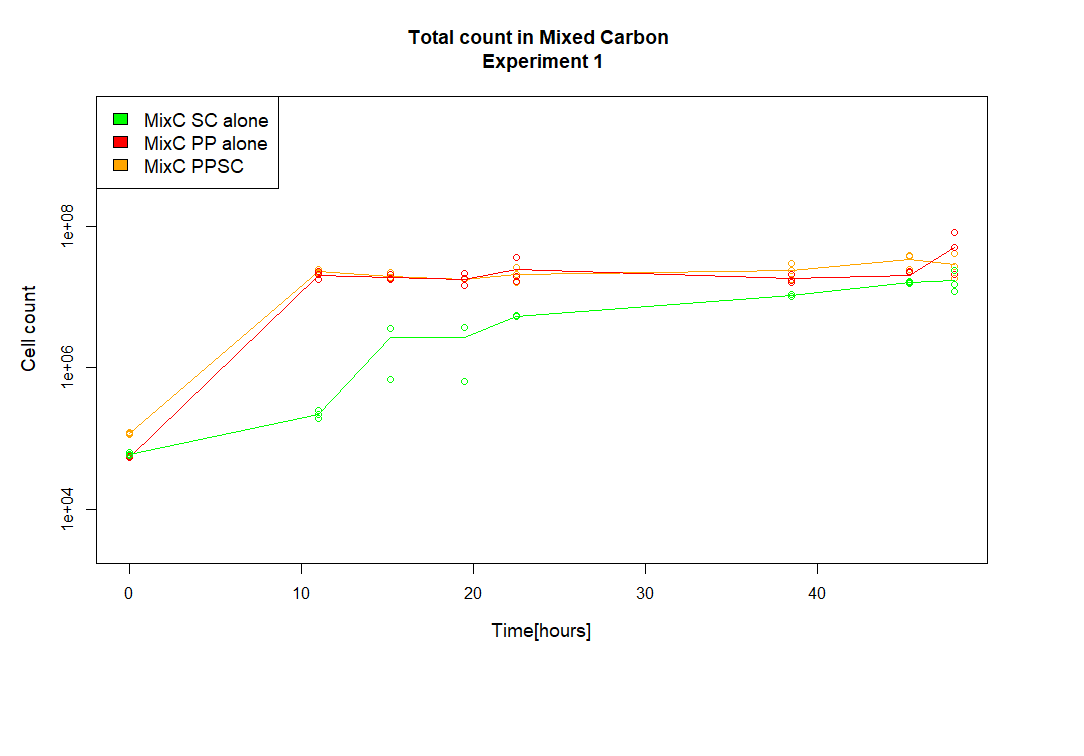
\includegraphics[width=9cm]{totcount_mixC1.PNG}
	\caption{Total count (SYTO-9 Count + mCherry count) of SC, PP and PPSC over time in a mixed carbon medium during the first week.}
	\label{totcountmixC1text}
\end{figure}

\begin{figure}
	\centering
	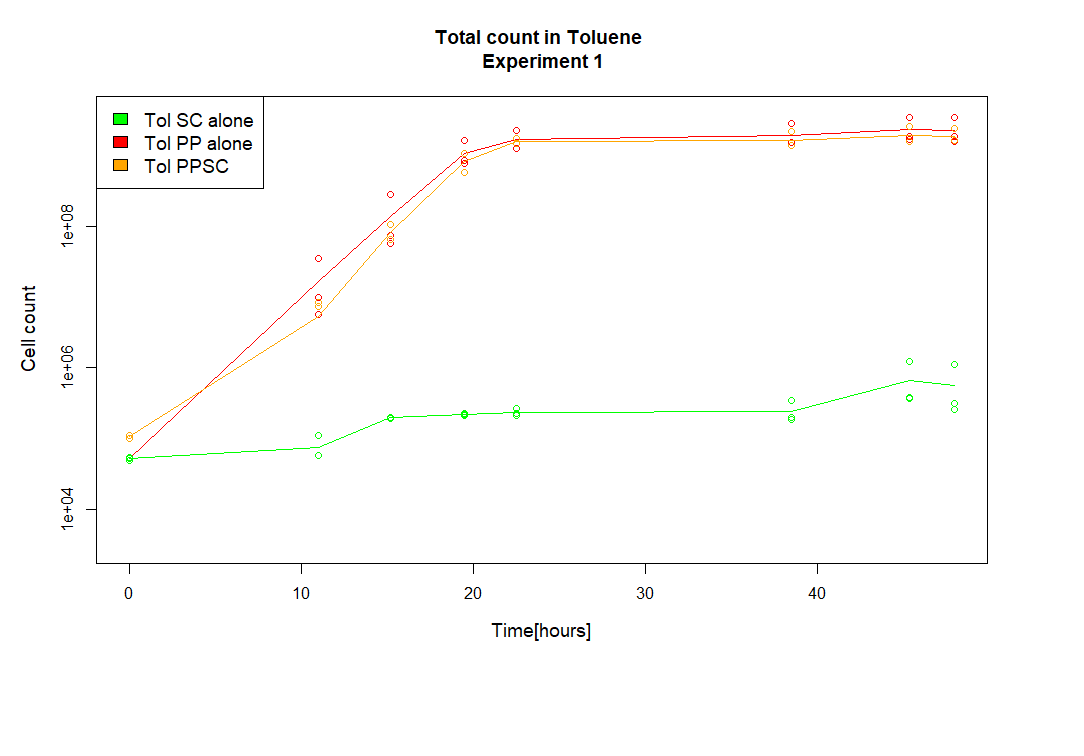
\includegraphics[width=9cm]{totcount_tol1.PNG}
	\caption{Total count (SYTO-9 count + mCherry count) of SC, PP and PPSC over time in a toluene only medium during the first week.}
	\label{totcounttol1text}
\end{figure}


\subsubsection{Sand Community}
The growth of the sand community in each treatment for the first week is represented in Fig. \ref{aucscw1} and \ref{SCgrowth1}.
There is an important interaction between the explicative variables (F = 26.62, df = 1, $p = 8.64\cdot 10 ^{-4}$).
In mixed carbon, SC grows similarly in presence or absence of PP (black and blue points).
In toluene however, the presence of PP allows for a 1000-fold difference on average (red and yellow points).
We conclude that the presence of PP affects SC differently depending on the media. In toluene, it allows for a better growth but has no effect in the mix carbon media. In addition, the effect of the media on SC is important in
\begin{figure}[H]
	\centering
	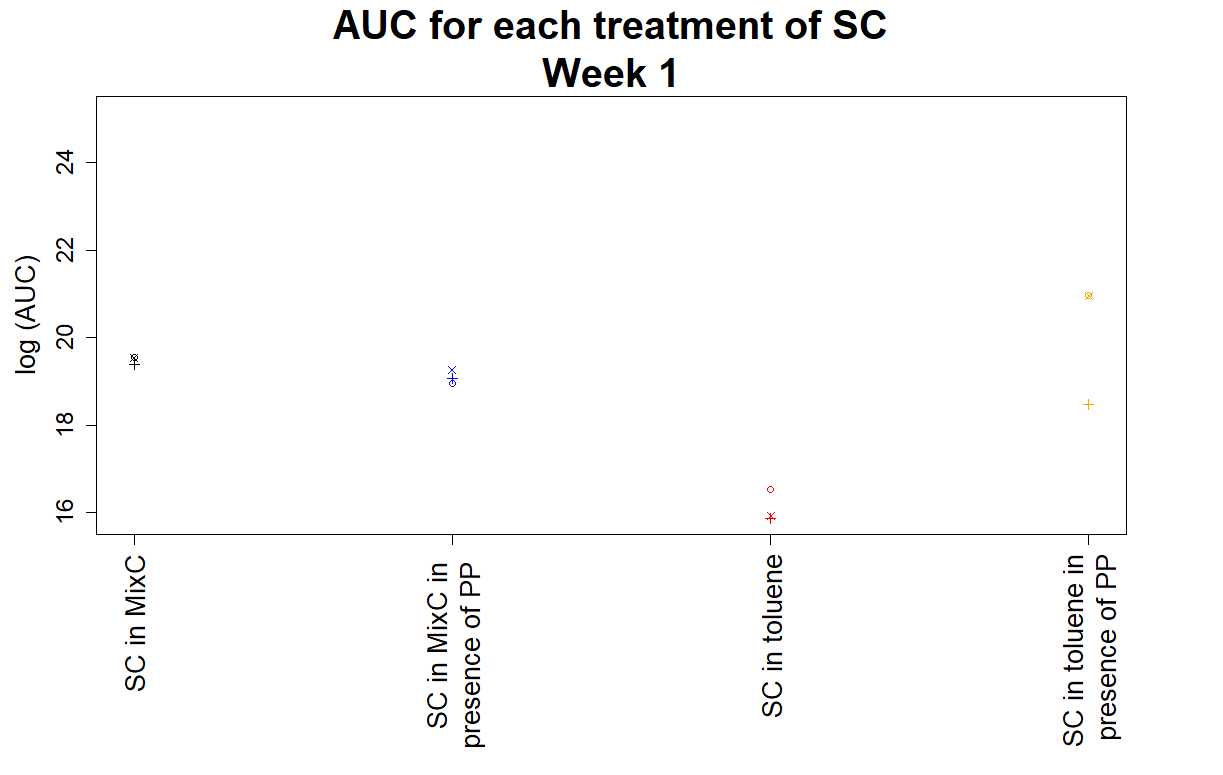
\includegraphics[width=9cm]{AUCsc1.png}
	\caption{Week 1 - SC : Each point represents one of the three replicates's AUC for each treatment.}
	\label{aucscw1}
\end{figure}%
\vspace{-0.4cm}
\begin{figure}[H]
	\centering
	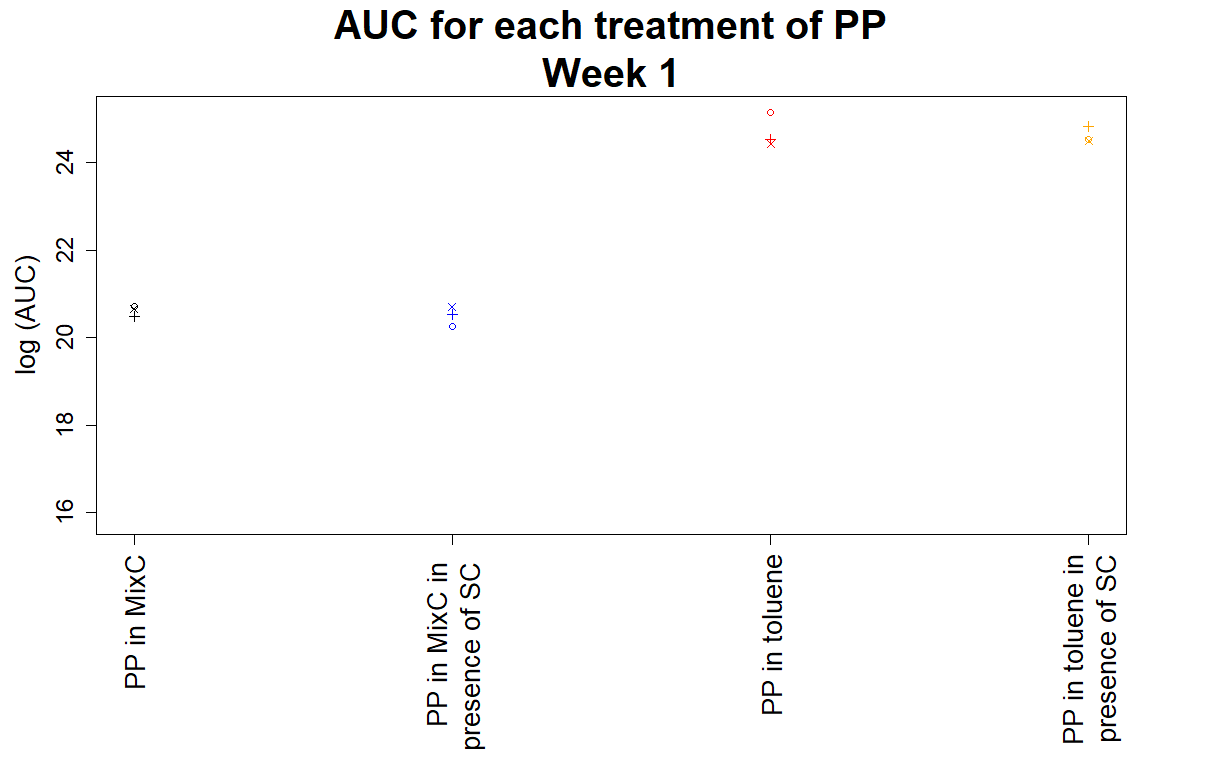
\includegraphics[width=9cm]{AUCpp1.png}
	\caption{Week 1 - PP : Each point represents one of the three replicates's AUC for each treatment.}
	\label{aucppw1}
\end{figure}
absence of PP. SC alone grows less in toluene than in mixed carbon.\newline
%There is an important difference between the media (F =907.30, df = 1, $p = 2.36 \cdot 10^{-6}$). It is clearly shown on the Fig. \ref{PPgrowth1} (red and yellow curves vs black and blue curves).
%In contrast, our data shows no significant difference due to the presence or absence of the sand community and no interaction.
%We conclude that SC has no effect on the growth of PP and that PP grows better in toluene only than in mixed carbon. It is certainly due the greater amount of carbon in the toluene media.

\subsubsection{Pseudomonas putida}
There is an important difference between the media (F =907.30, df = 1, $p = 2.36 \cdot 10^{-6}$). It is clearly shown on the Fig. \ref{aucppw1} and \ref{PPgrowth1} (red and yellow curves/points vs black and blue curves/points)).
In contrast, our data shows no significant difference due to the presence or absence of the sand community and no interaction.
We conclude that SC has no effect on the growth of PP and that PP grows better in the Toluene medium than in the mix carbon medium. It could be due to the greater amount of carbon in the toluene media.



%\begin{figure}[H]
%	
%	\begin{subfigure}{.5\textwidth}
%		\centering
%		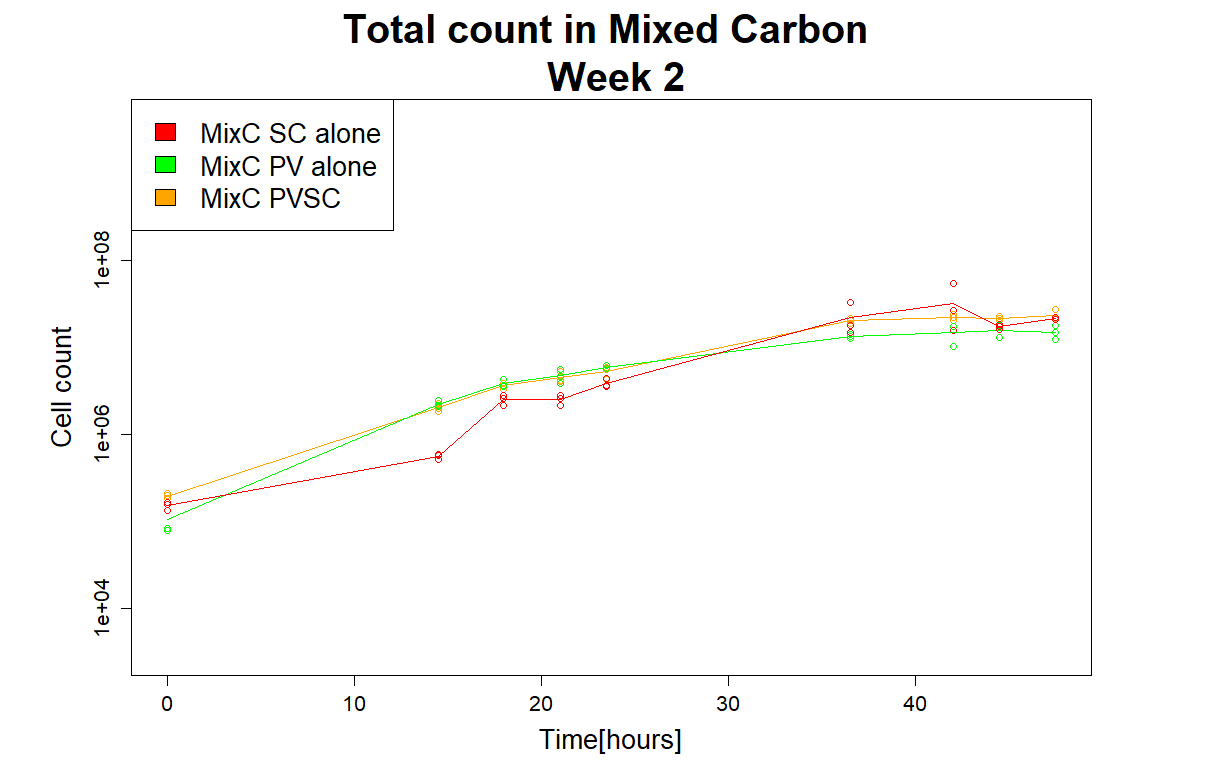
\includegraphics[width=9cm]{totcount_mixC2.PNG}
%		\caption{}
%		\label{totcountmixC2text}
%	\end{subfigure}
%	\begin{subfigure}{.5\textwidth}
%		\centering
%		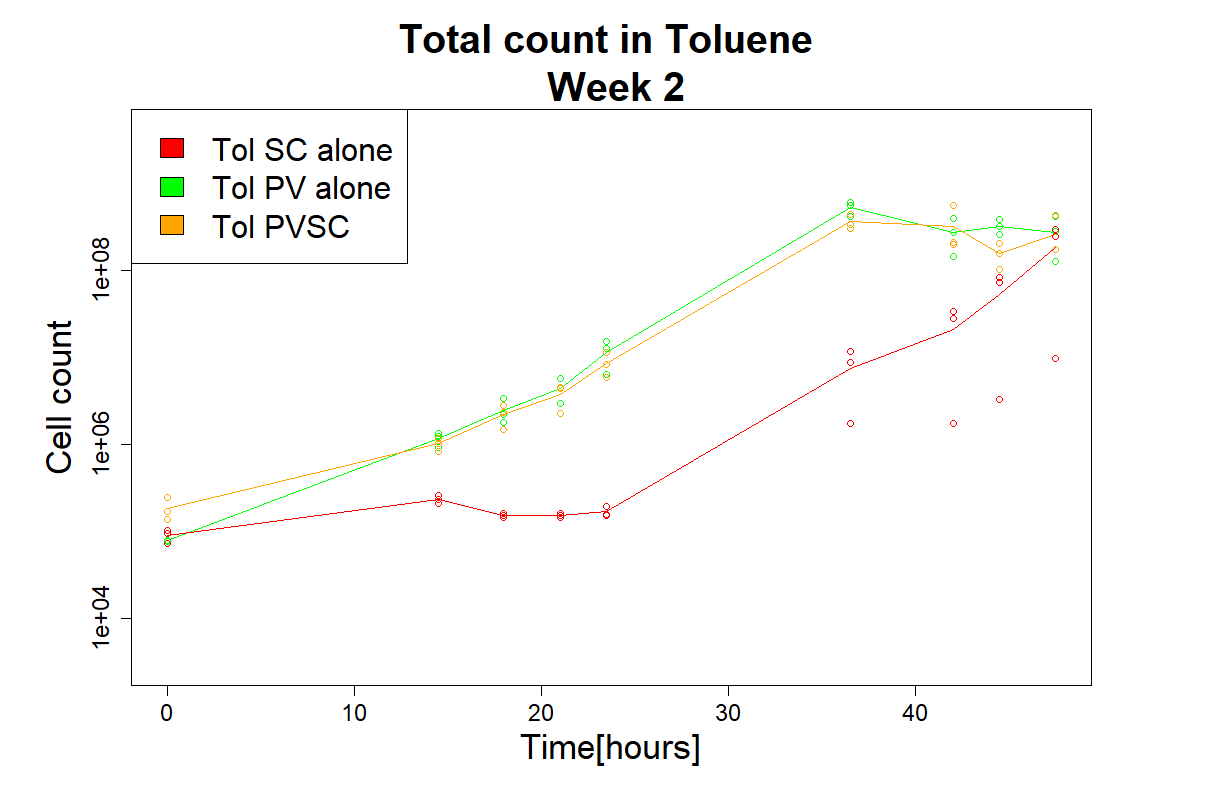
\includegraphics[width=9cm]{totcount_tol2.PNG}
%		\caption{}		
%		\label{totcounttol2text}
%	\end{subfigure}
%	\caption{Fig. \ref{totcountmixC2text}: Total count (SYTO-9 Count + mCherry count) of SC, PV and PVSC over time in a mixed carbon medium during the second week. Fig. \ref{totcounttol2text} : Total count (SYTO-9 count + mCherry count) of SC, PV and PVSC over time in a toluene only medium during the second week.}
%	\label{totcount2}
%	
%\end{figure}


\subsection{Week 2 $\textendash$ SC, PV, PVSC}

\subsubsection{Total cell count comparison}
The total cell count over time is represented on Fig. \ref{totcountmixC2text} and \ref{totcounttol2text}, the conclusion is the same as in the first week. It shows no signs that growing PV and SC together influences the growth of the overall population nor the total cell count after 48 hours, in a mixed carbon or toluene media.\newline

\begin{figure}[H]
	\centering
	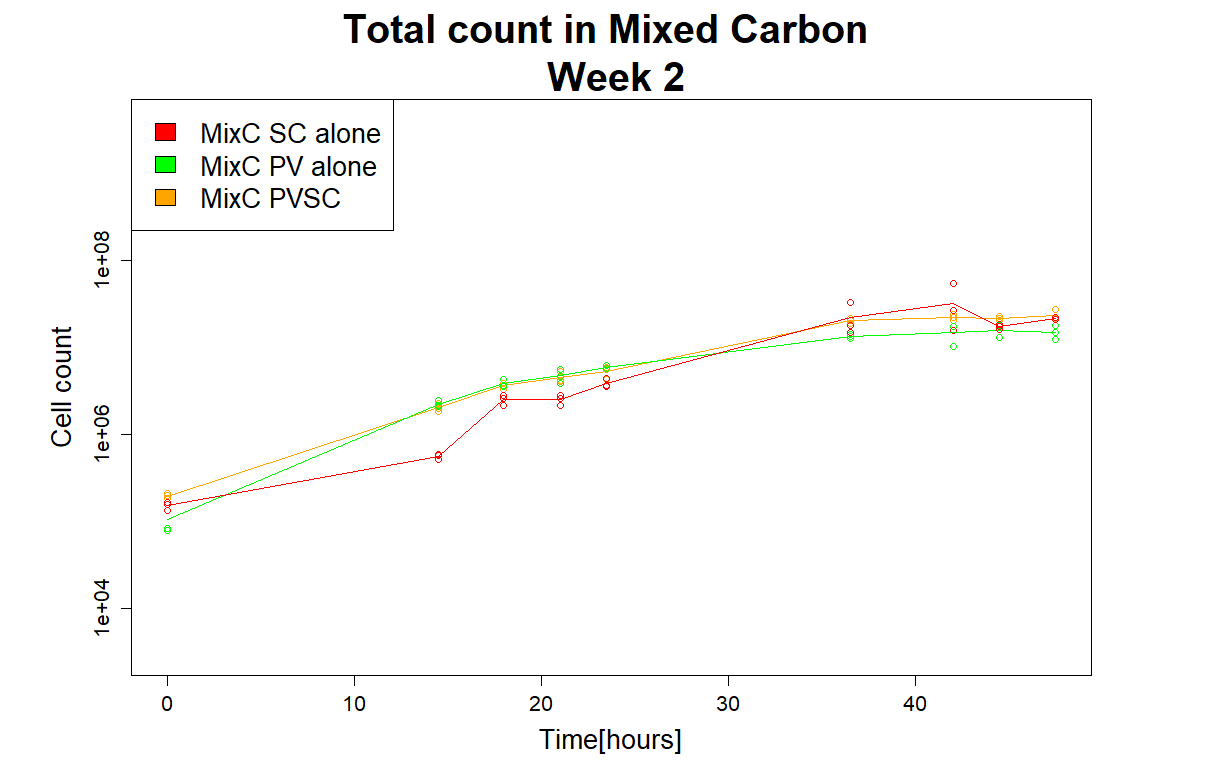
\includegraphics[width=9cm]{totcount_mixC2.PNG}
	\caption{Total count (SYTO-9 Count + mCherry count) of SC, PV and PVSC over time in a mixed carbon medium during the second week.}
	\label{totcountmixC2text}
\end{figure}
\vspace{-0.4cm}
\begin{figure}[H]
	\centering
	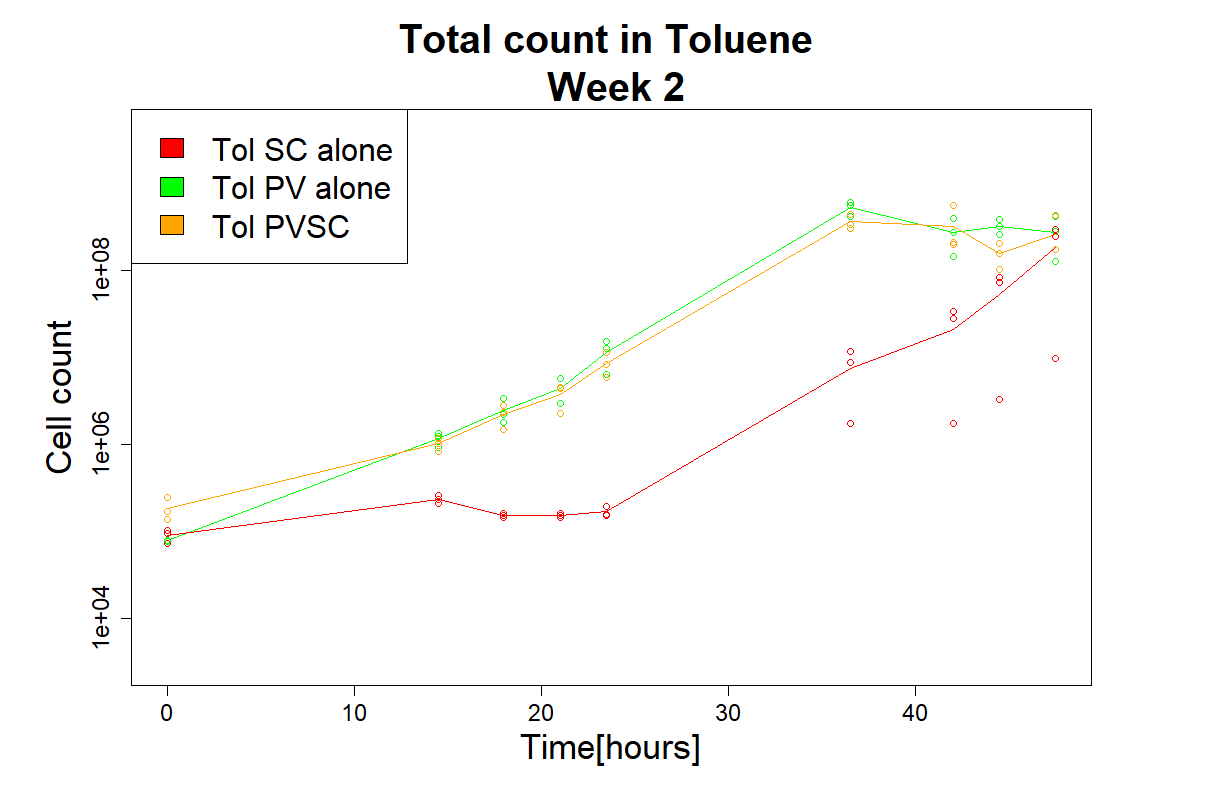
\includegraphics[width=9cm]{totcount_tol2.PNG}
	\caption{Total count (SYTO-9 count + mCherry count) of SC, PV and PVSC over time in a toluene only medium during the second week.}
	\label{totcounttol2text}
\end{figure}
\subsubsection{Sand Community}
The growth of the sand community in each treatment for the second week is represented in Fig. \ref{aucscw2} and \ref{SCgrowth2}.
In contrast with the first week, SC was able to grow in toluene (red curves/points). It is not surprising, as a community extracted from sand is typically composed of many kinds of bacteria. It is likely that at least one of them can degrade a given carbon source. But it shows that SC behaved differently from one week to another and thus cannot be considered identical. Therefore, we won't be able to compare the results from the two weeks. 
The Anova on the area under the curve shows no significant effect of any explicative variables, but we believe the results could be different if we continued the culture for a day because we can see on the growth graph that SC alone is still in exponential growth at 48 hours in toluene. It is plausible that with a few more timepoints, SC would grow better alone than in presence of PV.\newline


\subsubsection{Pseudomonas veronii}
The growth of PV in each treatment is represented in Fig. \ref{aucpvw2} and \ref{PVgrowth2}.
As in the first week, there is an important difference of growth between the media (F = 784.71, df = 1, $p = 2.85 \cdot 10^{-9}$). PP grew about a hundred-fold better in toluene (red and orange) than in mixed carbon (black and blue curves/points).
One can also notice that PP grew slightly less in presence of SC, in both media (blue and yellow compared to black and red curves/points). The difference in area under the curve is significant (F = 5.56, df = 1, $p = 0.046$). While not being as significant as our other results, it could indicate some competition between them in this type of culture. It seems plausible, knowing from previous experiments that PV grows a bit slower than PP and in this experiment some bacteria from the sand community were able to grow on toluene.
\newline

\begin{figure}[H]
	\centering
	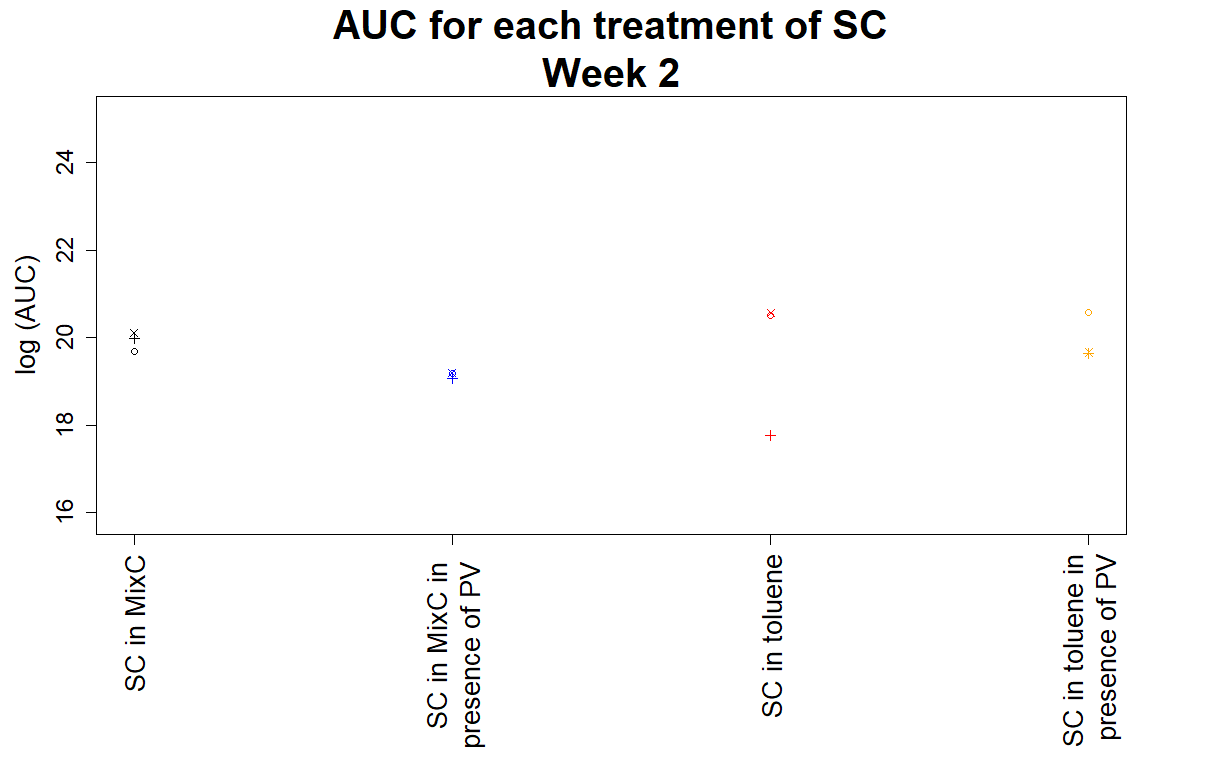
\includegraphics[width=9cm]{AUCsc2.png}
	\caption{Week 2 - SC : Each point represents one of the three replicates's AUC for each treatment.}
	\label{aucscw2}
\end{figure}%
\vspace{-0.3cm}
\begin{figure}[H]
	\centering
	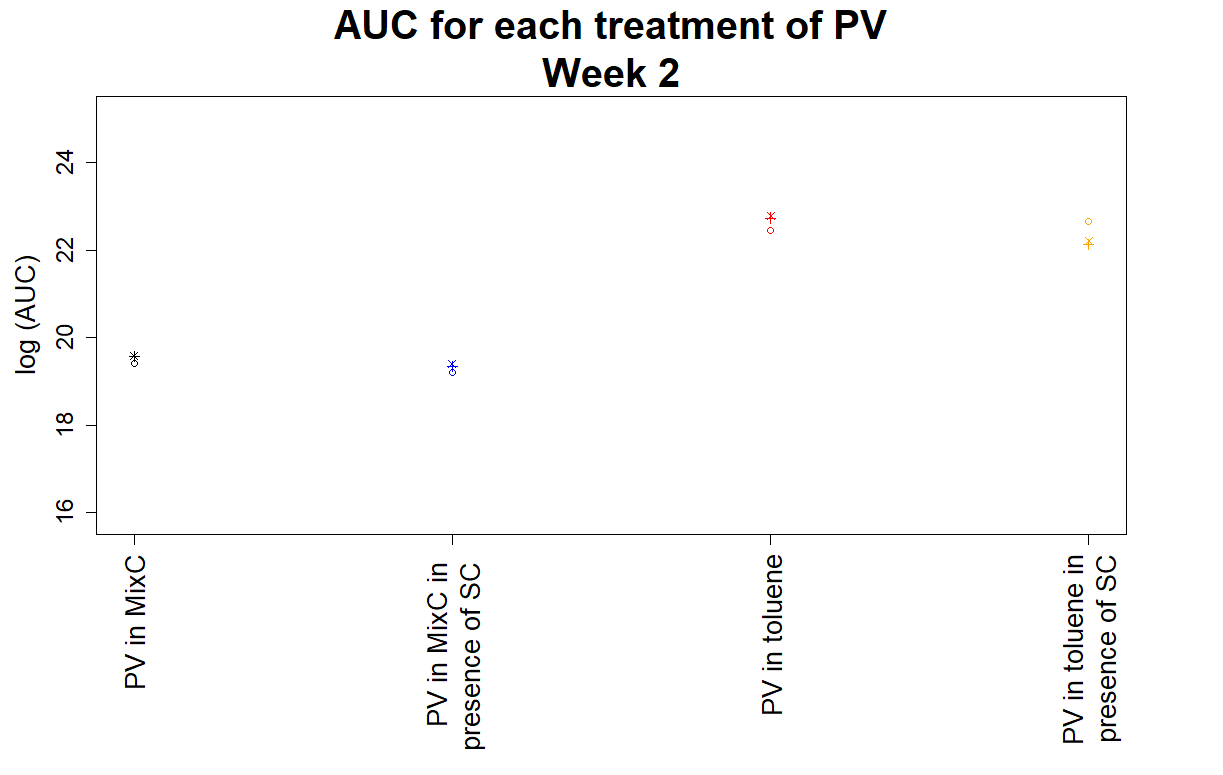
\includegraphics[width=9cm]{AUCpv2.png}
	\caption{Week 2 - PV : Each point represents one of the three replicates's AUC for each treatment.}
	\label{aucpvw2}
\end{figure}

\section{Discussion}
%While these results are promising, further analysis and plotting were carried out to ensure reliability of our results. 
%The first drawback of the design we noticed is the proportion of SC cells compared to PP or PV  (Fig. \ref{barplot}). We see that the proportion of SC is low compared to the overall population ($\cong 5\%$). This would be a problem in a bioremediation context because the original community was almost completely replaced.


%\begin{figure}
%	\centering
%	 
%	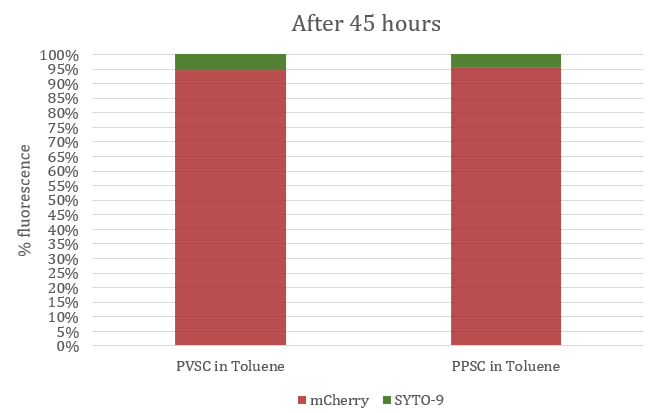
\includegraphics[width=8cm]{problem_barplot.PNG}
%	\caption{Proportion of red and green fluorescence in the PV + SC and PP + SC cultures in toluene.}
%	\label{barplot}
%	  
%\end{figure}
%To solve this problem, we would like to analyse this further by trying different culture conditions. Firstly, we would try to have a mixed carbon with toluene substrate. Secondly, it would be great to vary toluene and carbon concentration. Third and final, we would like our conditions to be as close to reality as possible. For example growing the cells in sand would certainly affect their growth and fitness.
%

%We noticed a slight drawback when we plotted the count of SYTO-9 stained cells over time, for PP alone and PPSC in toluene in Fig. \ref{problemw1} and \ref{problemw2}. 

\subsection{mCherry issue}
Further analysis was carried out to ensure the reliability of our promising results. It brought a slight drawback to light.
Some cells were detected in the SYTO-9 only gate in PP alone and PV alone cultures in both media (Fig. \ref{problemflow}). Fig. \ref{problemflow1} is a representation of PP alone in toluene, and Fig. \ref{problemflow2} of PPSC in toluene, both at the same timepoint. These graphs are almost identical, and more importantly, both show an important count in the SYTO-9 only gate (Fig. \ref{problemw1}, Fig. \ref{problemw2}). We also observe this phenomenon with PV alone.
This is quite surprising, knowing that both PP and PV were tagged with mCherry. This protein emits a
red fluorescence and should cause an upwards shift in the fluorescence graph (as explained in Fig. \ref{scatter1} and \ref{scatter2}) and bring these cells in the mChe + SYTO-9 gate.

Our hypothesis is that some PP/PV cells died, but weren’t lysed. Their DNA is still nicely protected  in the cell and can be stained by SYTO-9. However, their metabolic activities stopped, reducing mCherry fluorescence. Without the red tag, these cells would shift downwards and into the SYTO-9 only gate. It renders differentiation between PP (or PV) and SC seemingly impossible because they both appear in the same gate. A multivariate analysis using PCA (Principal Component Analysis) and K-means clustering was performed to try to differentiate the two controls (PP alone, SC alone) with other factors (forward-scatter and side-scatter for example), but to no avail.

This issue makes us question whether the significant increase in AUC in the SYTO-9 only in PPSC compared to SC alone is due to an increase of the number of SC or to the presence of PP cells presenting low red fluorescence values. 

To circumvent this problem, another tagging method unaffected by cell death could be used (Fig. \ref{antibody}). For example, a highly specific antibody to \textit{Pseudomonas putida} could be engineered. A secondary antibody, this time linked to a fluorescent protein would bind the first one and therefore mark all \textit{Pseudomonas putida} cells. This would allow a better differentiation of our communities.



\begin{figure}
		\centering
		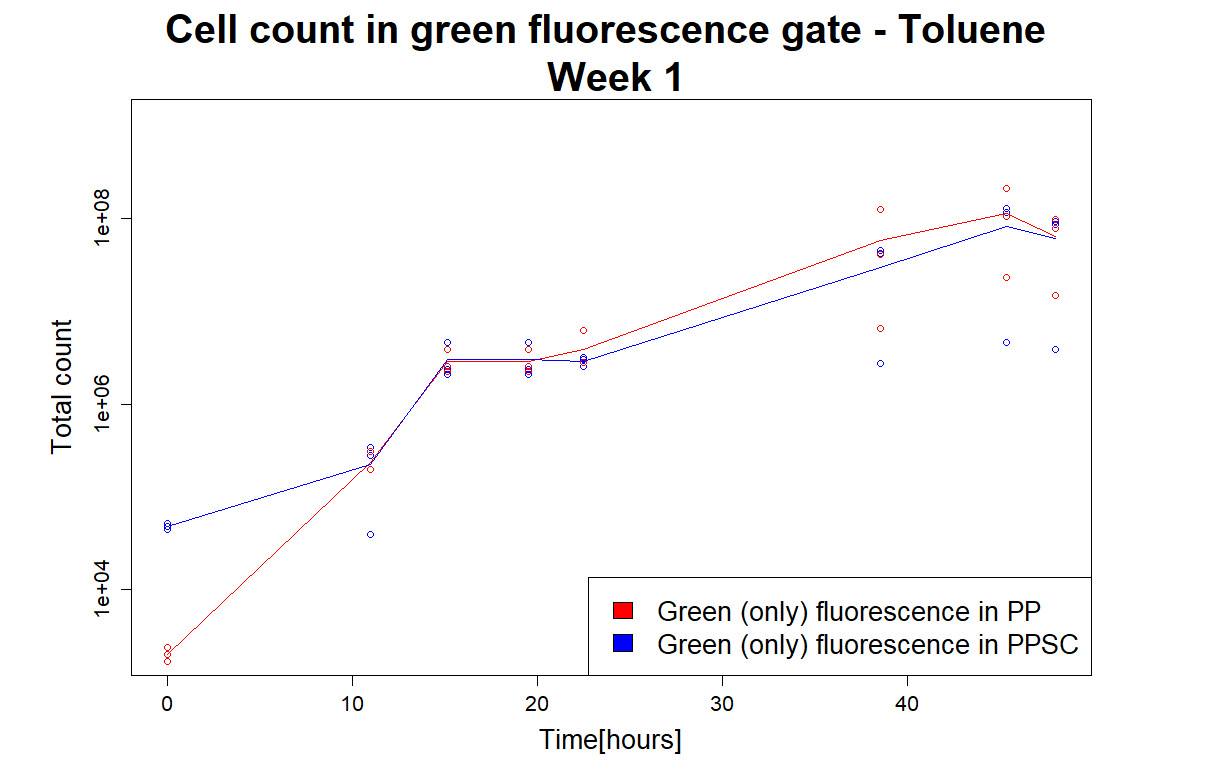
\includegraphics[width=9cm]{problemw1.PNG}
		\caption{Total count of green stained cells in toluene for PP alone and PP with SC during week 1. It showed no significant differences. Each point is a replicate, and each line is the mean of the corresponding replicates.}
		\label{problemw1}
\end{figure}

\begin{figure}
		\centering
		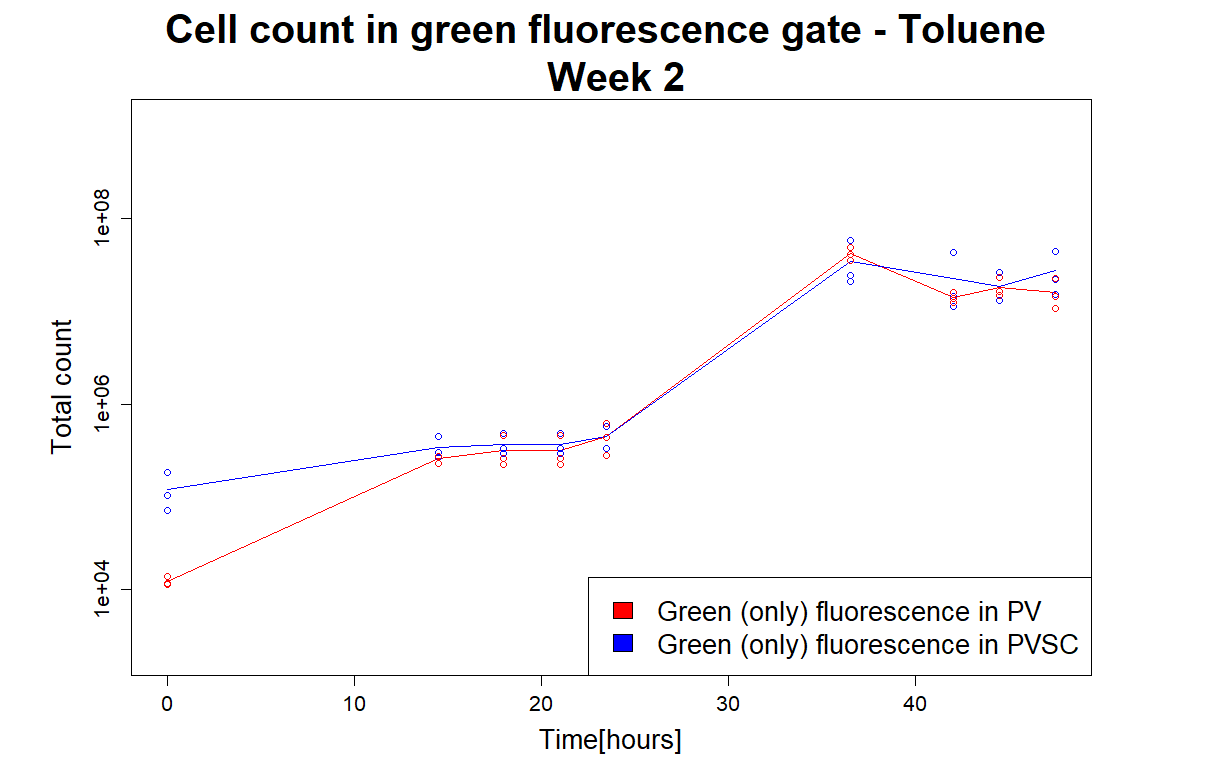
\includegraphics[width=9cm]{problemw2.PNG}
		\caption{Total count of green stained cells in toluene for PV alone and PV with SC during week 2. It showed no significant differences. Each point is a replicate, and each line is the mean of the corresponding replicates.}
		\label{problemw2}

%\caption{Fig. \ref{problemw1} : Total count of green stained cells in toluene for PP alone and PP with SC during week 1. It showed no significant differences. Fig. \ref{problemw2} : Total count of green stained cells in toluene for PV alone and PV with SC during week 2. It showed no significant differences.}
%\label{problemsyto}
  
\end{figure}

\begin{figure}
	\hspace{-0.3cm}
	\begin{subfigure}{.25\textwidth}
		\centering
		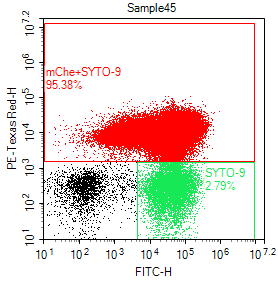
\includegraphics[width=4.3cm]{PP3T5.png}
		\caption{}
		\label{problemflow1}
	\end{subfigure}%
	\begin{subfigure}{.22\textwidth}
		\centering		
		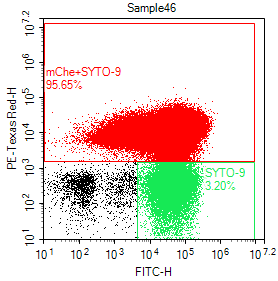
\includegraphics[width=4.3cm]{PPSC1T5.png}
		\caption{}
		\label{problemflow2}				
	\end{subfigure}
	\caption{Scatterplot of a stained PP sample(Fig. \ref{problemflow1}) besides a stained PPSC sample (Fig. \ref{problemflow2}). They look very similar. A lot of PP seem to have lost mCherry (red) fluorescence and have shifted downwards (Fig. \ref{problemflow1}) and look like the supposed SC cells in Fig. \ref{problemflow2}.  }
	\label{problemflow}
\end{figure}	


% Indeed, the fact that we get a green-only fluorescence in PP and PV alone is surprising, knowing that both PP and PV were tagged with mCherry, which emits a red fluorescence and causes an upwards shift in the fluorescence graph (as explained in Fig. \ref{scatter1} and \ref{scatter2}). Moreover, the number of green-fluorescent cells in PP or PV alone looks a lot like the number in PPSC (Fig. \ref{problemw1}) or PVSC (Fig. \ref{problemw2}).
% 
%It is even more visible in Fig.\ref{problemflow}. Fig.\ref{problemflow1} is a representation of PP alone in toluene, and Fig.\ref{problemflow2} of PPSC in toluene. These graphs are almost identical, and both show a green-only fluorescence.
% 
%
%Our hypothesis is that some PP/PV cells died, but weren’t lysed. Their DNA being still nicely protected they could be stained by SYTO-9. However, their metabolic activities stopped, reducing mCherry fluorescence. Without the red tag, these cells would shift downwards and remain in the SYTO-9 only gate and can't be differentiated from the SC cells.


%\subsection{Improvements}



%Another point that could be interesting to change is the initial concentration of PP and PV. Indeed we used $10^{6}$ cells of SC and $10^{6}$ cells of PP or PV. Maybe by reducing the initial concentration of PP/PV, we could reduce their competition with SC over resources, and therefore observe a better growth for SC in toluene media. 
%
%In addition, we inoculated the media with the same number of PP or PV with SC and haven't considered the fact that SC community is composed of different bacterial species.
%The high quantity of a single strain may have made it easier for them  to outgrow SC over time. 

%Finally, as often in the lab, our results seem to unveil more questions than answers. We would have liked, if time allowed it, to perform additional experiments proposed above. Because in the present state, we got interesting results, but due to some unforeseeable events, we cannot be certain that they are not artefacts due to the issue differentiating the cells we mentioned before. 
%
%Finally, the results of our study open new questions for which we need to perform additional experiments, such as those described above. The issue with this staining technique might carry some artefacts that should be considered in data interpretation.

\subsection{Bacterial interactions}
To summarise, growing PP or PV with SC shows no effect on the total cell count compared to growing PP / PV alone. 
\begin{figure}[H]
	\centering
	
	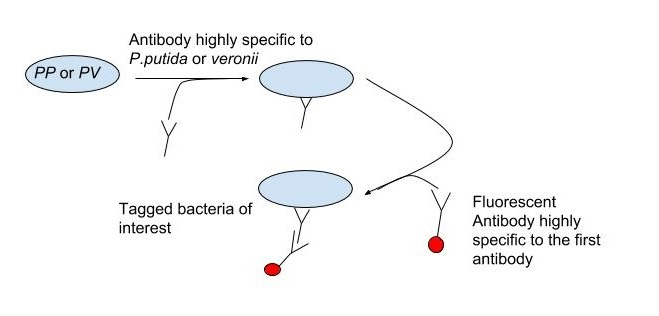
\includegraphics[width=8.5cm]{antibodytag.jpg}
	\caption{Fluorescent antibody tagging, as an alternative to mCherry in this experiment}
	\label{antibody}
	
\end{figure}
If we assume this tagging issue is negligible, we can infer on the growth of each population separately within each treatment. In the first week, the data indicates that the presence of PP affects SC differently depending on the media (Interaction: F = 26.62, df = 1, $p = 8,64 \cdot 10^{-4}$).  In toluene, it allows a better growth but has no effect in the mix carbon media.  There is an important effect of the media in absence of PP: SC alone grows significantly less in toluene than in mixed carbon. Furthermore, PP shows an important difference in AUC between the media (F =907.30, df = 1, $p = 2.36 \cdot 10^{-6}$) and no difference due to the presence of SC.  

During the second week, SC behaved differently: it was able to grow in the toluene media, even alone. No significant effect of the media nor of the addition of PV were highlighted by the Anova. 
Similarly to PP, PV had a better growth in toluene than in mixed carbon (F = 784.71, df = 1,
$p = 2.85 \cdot 10^{-9}$). This time however, there was a significant reduction of the number of PV in presence of SC in toluene (F =5.56, df = 1, $p = 0,046$). While not being as significant as our other results, it seems to indicate some competition between them in this type of culture.

It might also be important to notice that even if the AUC of the SYTO-9 gate in PPSC is significantly higher than in SC alone, the proportion of SC in PPSC is very low (about 5\%).

To study more deeply these interaction, it might be interesting to change the initial concentration of PP and PV. Indeed we used 10\textsuperscript{6} cells of SC and 10\textsuperscript{6} cells of PP or PV. Maybe by reducing the initial concentration of PP/PV, we could reduce their competition with SC over resources, and therefore observe a better growth for SC in toluene media. 

In addition, we inoculated the media with the same number of PP or PV with SC and haven’t considered the fact that SC community is composed of different bacterial species. The high quantity of a single strain (PP or PV) may have made it easier for them to outgrow SC over time. 

\subsection{Back to context}
In many bioaugmentation experiments, one of the main challenges is the survival of the inoculated strain in presence of a bacterial community \cite{bouchez} \cite{oldarticle}, particularly in absence of pollutant \cite{nodrawback}.

In our experiments, PP and PV were able to grow in both media in presence or absence of SC. This led us to think that PP and PV would be interesting candidates for bioaugmentation, especially as they have no problem growing with SC in mixed carbon. 

As PV showed a significantly lower growth on average in toluene in presence of SC than PP, it would be tempting to say that PP would be an even better candidate. However, as said in \textit{Results} section \textit{B2}, our data isn't totally reliable to compare the two strains, as the SC extracted the two weeks behaved differently. It would be good to test PP and PV on the same SC. 

Further experiments would be required to know if this is also true in a sand medium (and not liquid medium) and especially over a longer period of time. Similar experiments could also be performed on different native communities. Also, it would be interesting to vary the concentration of toluene in these experiments. 

\subsection{Conclusion}

In the present state, our study shows interesting results. However, the issue with this staining technique might carry some artefacts that should be considered in data interpretation. If time had allowed it, we would have liked to perform the additional experiments proposed above to solve this issue.
 

%\addtolength{\textheight}{-12cm}  % This command serves to balance the column lengths
                 % on the last page of the document manually. It shortens
                 % the textheight of the last page by a suitable amount.
                 % This command does not take effect until the next page
                 % so it should come on the page before the last. Make
                 % sure that you do not shorten the textheight too much.

%%%%%%%%%%%%%%%%%%%%%%%%%%%%%%%%%%%%%%%%%%%%%%%%%%%%%%%%%%%%%%%%%%%%%%%%%%%%%%%%



%%%%%%%%%%%%%%%%%%%%%%%%%%%%%%%%%%%%%%%%%%%%%%%%%%%%%%%%%%%%%%%%%%%%%%%%%%%%%%%%



%%%%%%%%%%%%%%%%%%%%%%%%%%%%%%%%%%%%%%%%%%%%%%%%%%%%%%%%%%%%%%%%%%%%%%%%%%%%%%%%



\section*{Acknowledgments}
Many thanks to Manupriyam Dubey and Andrea Vucicevic for their help in the lab and the design, their presence and support throughout this experiment. We also wish to thank Sara Mitri and Frédéric Schütz for their precious advices. 



\printbibliography
\vspace*{\fill}
\textit{APPENDIX A on next page}
\clearpage
\section*{Appendix A}

\begin{figure}[H]
	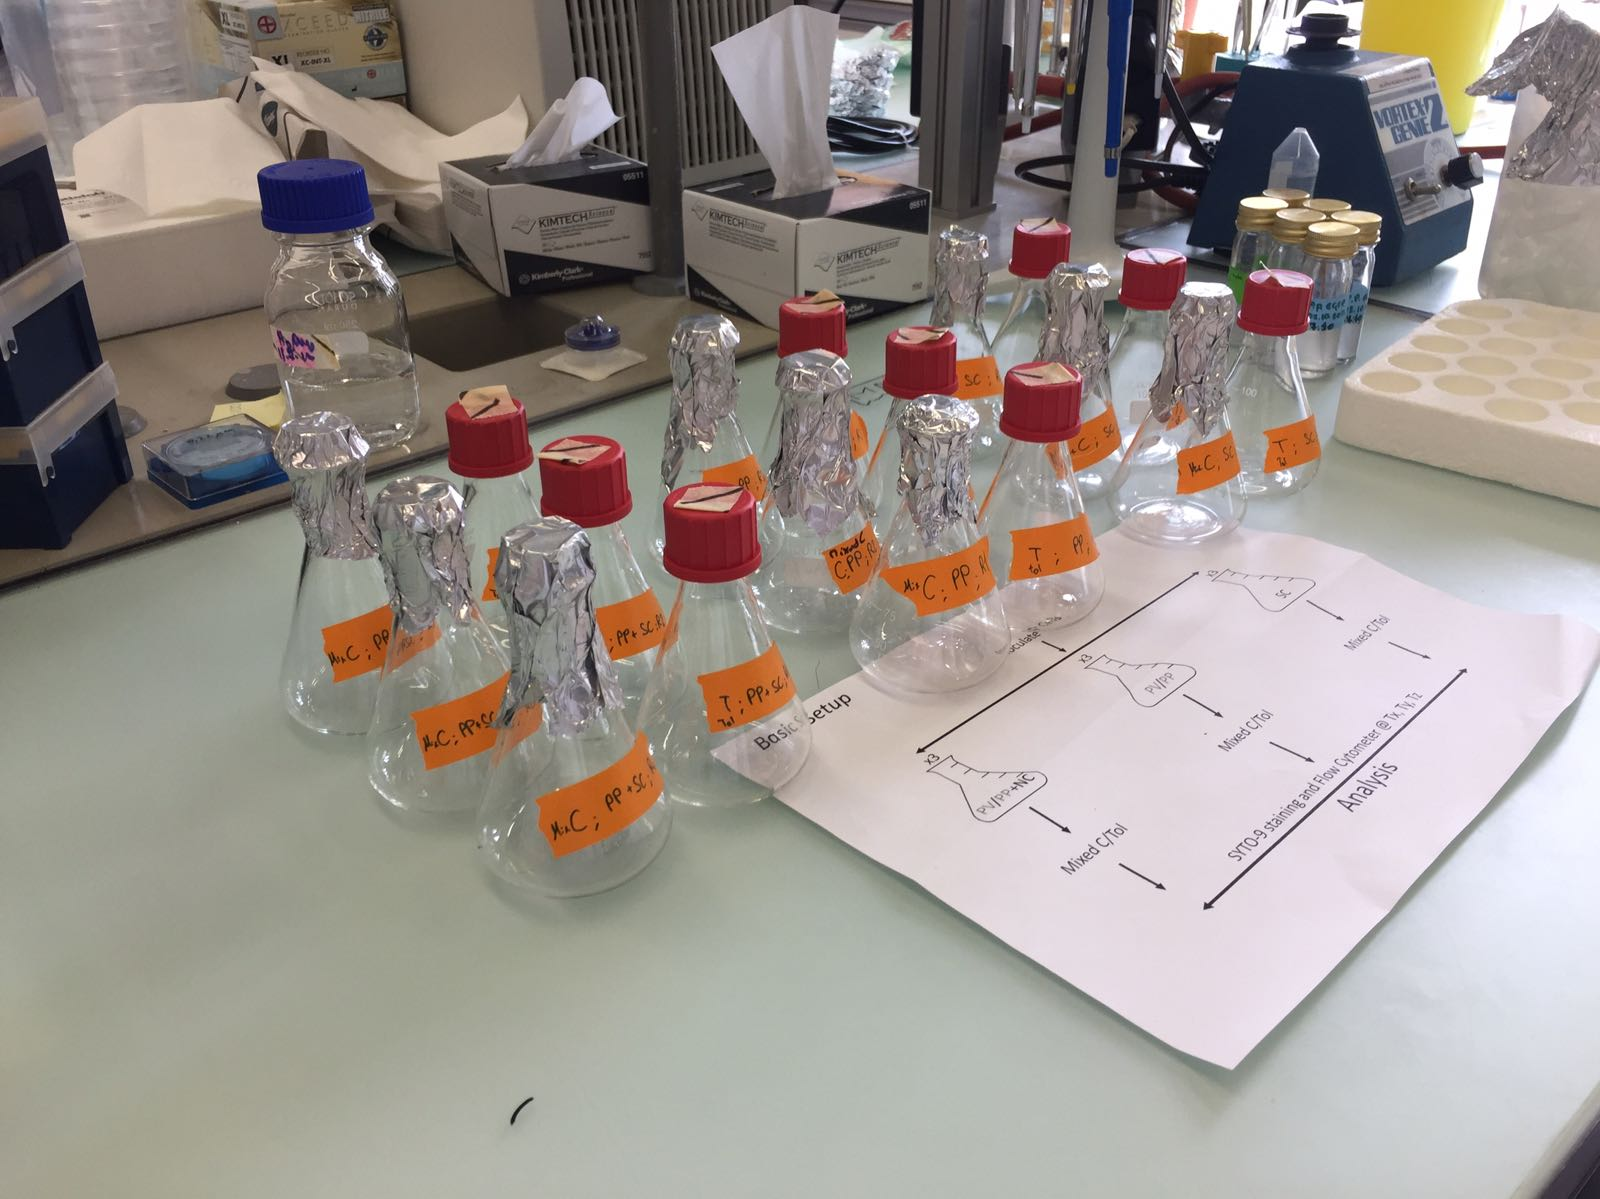
\includegraphics[width=8.5cm]{flasks.jpg}
	\caption{Flasks of week 1. The ones with the aluminum foil caps contain the mixed carbon medium and are not sealed. The ones with the red cap contain the toluene (see the sealed tip inside) and are sealed to avoid toluene leaks and loss of pollutant.}
	\label{flasks}
\end{figure}

%$\displaystyle\frac{\text{nbr of colonies } \cdot \text{ dilution factor } \cdot \text{ 100 $\mu$L of 1mL total}}{\text{estimated orginal number of cells}} = $\\
%
%
%$\displaystyle\frac{1109 \cdot 25 \cdot 10}{2\cdot 10^{9}}= 1.39 \cdot 10 ^{-4}$

\vspace*{\fill}
\textit{APPENDIX B on next page}
\clearpage
\newgeometry{bottom=1.5cm,top=1.5cm}
\begin{landscape}
	
	
	\begin{figure}
		\section*{Appendix B}
		
		\flushleft
		\begin{subfigure}{.47\textheight}
			\centering
			
			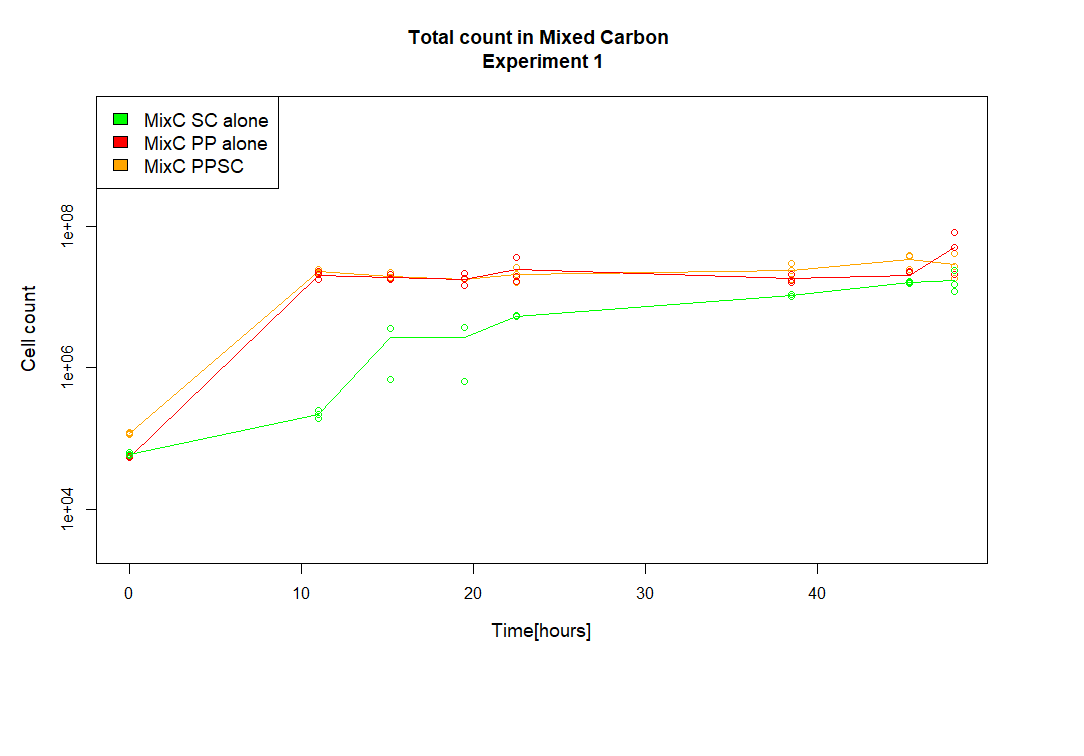
\includegraphics[width=7.71cm]{totcount_mixC1.png}
			%	\phantomsubcaption
			\caption{}
			%	\caption{Growth curves of total count in Mixed Carbon, Experiment 1 }
			
			\label{totcountmixC1}
		\end{subfigure}%
		\begin{subfigure}{.47\textheight}
			\centering
			
			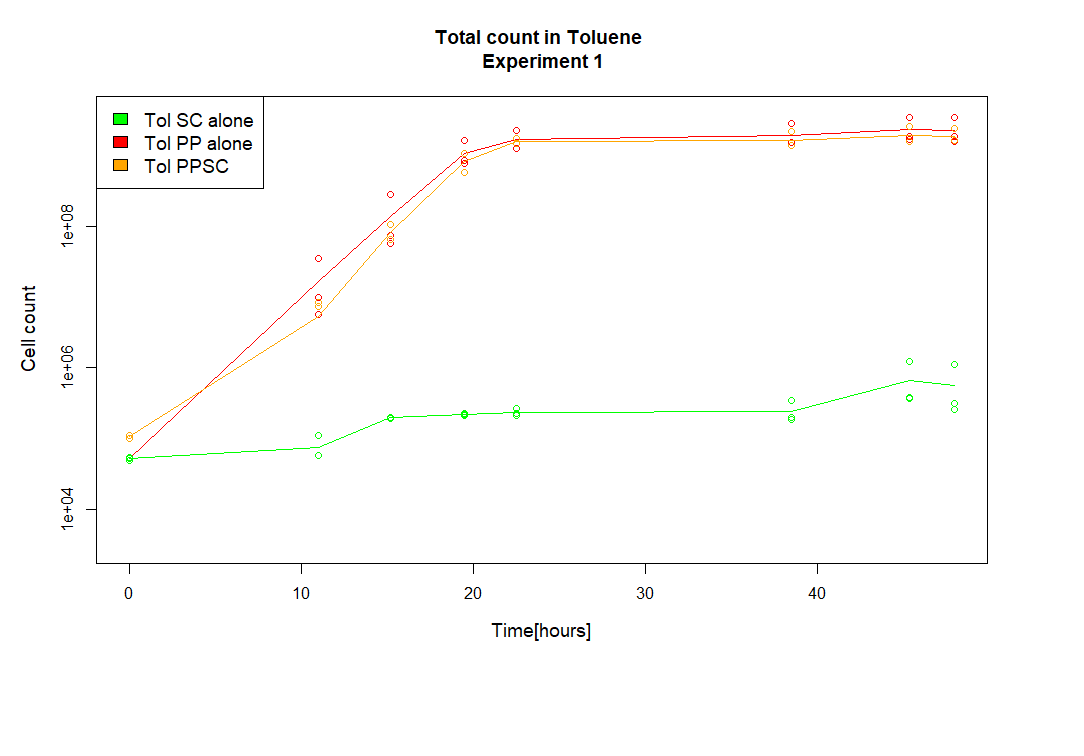
\includegraphics[width=7.71cm]{totcount_tol1.png}
			%		\phantomsubcaption
			\caption{}
			%		\caption{Growth curves of total count in toluene, Experiment 1 }
			\label{totcounttol1}
		\end{subfigure}%	
		\begin{subfigure}{.47\textheight}
			\centering
			
			%\vspace{-0.1cm}
			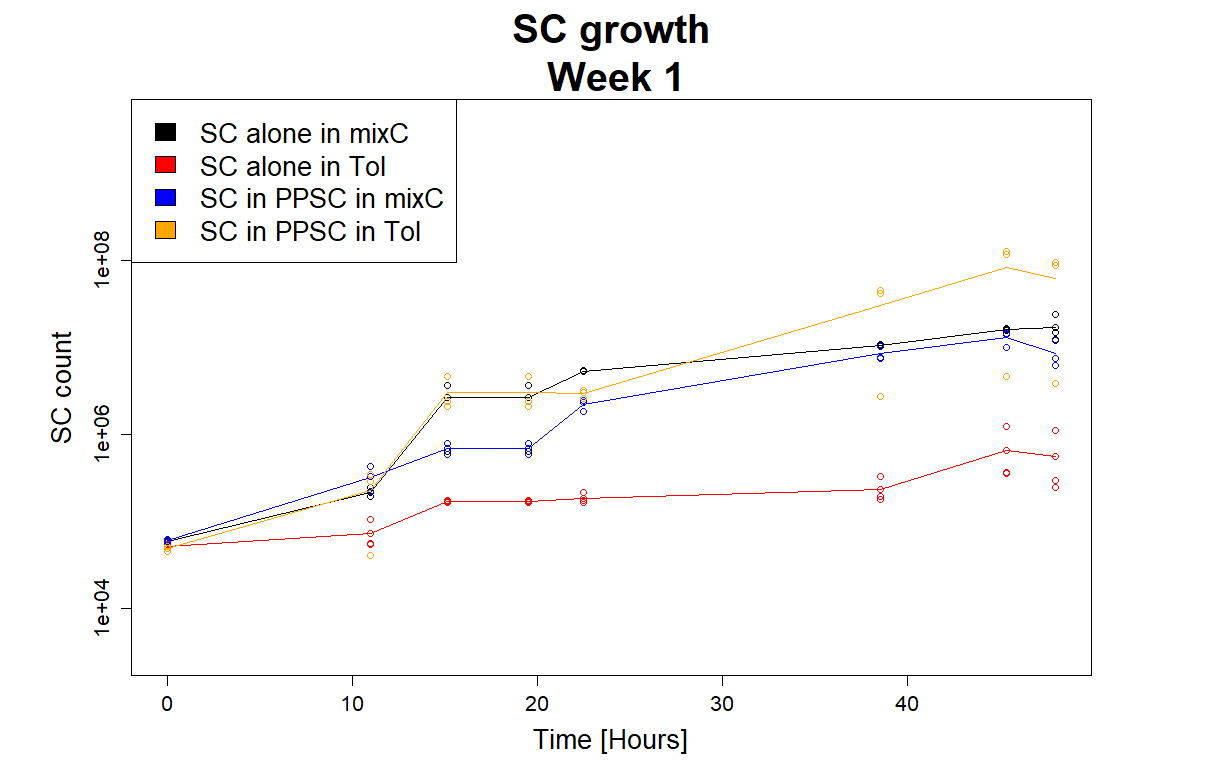
\includegraphics[width=7.71cm]{SCgrowth1.png}
			%		\phantomsubcaption
			\caption{}
			%		\caption{SC Growth curves, Experiment 1}
			\label{SCgrowth1}
		\end{subfigure}%
		\begin{subfigure}{.47\textheight}
			\centering
			\vspace{0cm}
			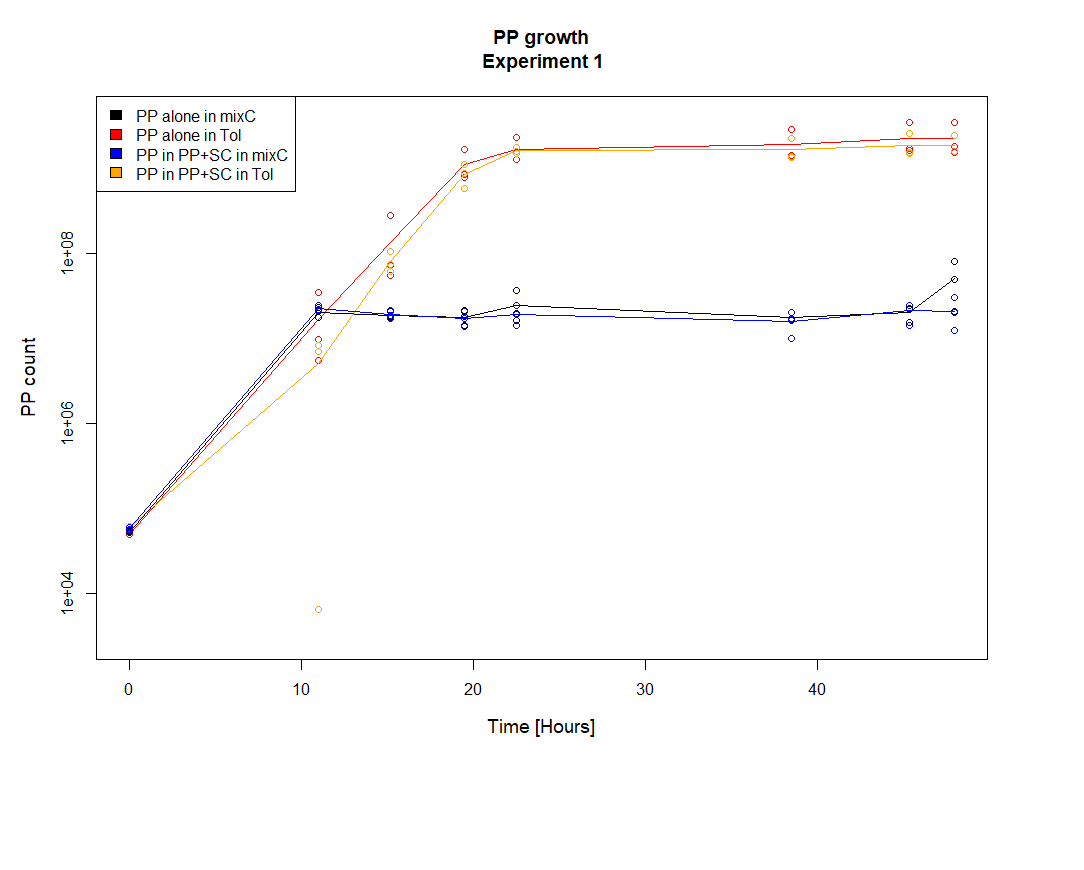
\includegraphics[width=7.71cm]{PPgrowth1.png}
			%			\phantomsubcaption
			\caption{}
			%		\caption{PP Growth curves, Experiment 1}
			\label{PPgrowth1}
		\end{subfigure}	
		\begin{subfigure}{.47\textheight}
			\centering
			
			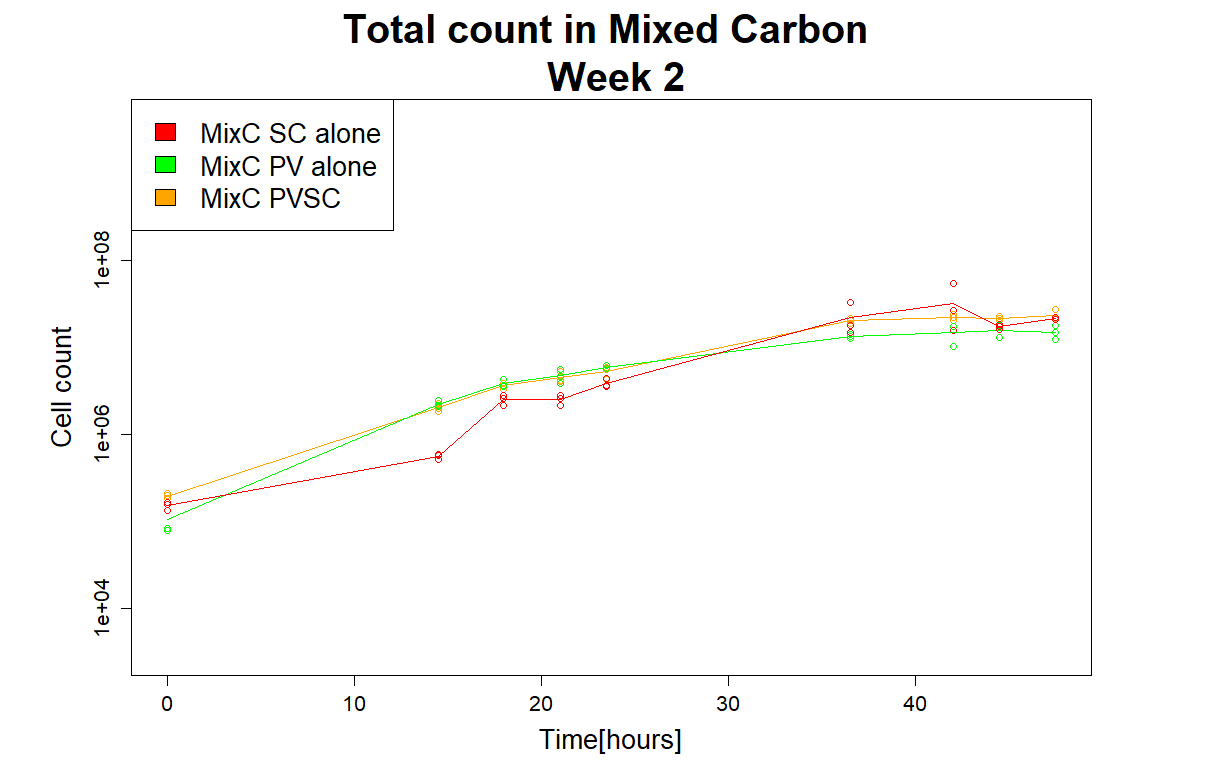
\includegraphics[width=7.71cm]{totcount_mixC2.png}
			%		\phantomsubcaption
			\caption{}
			%		\caption{Growth curves of total count in Mixed Carbon, Experiment 2}
			\label{totcountmixC2}
		\end{subfigure}%
		\begin{subfigure}{.47\textheight}
			\centering
			
			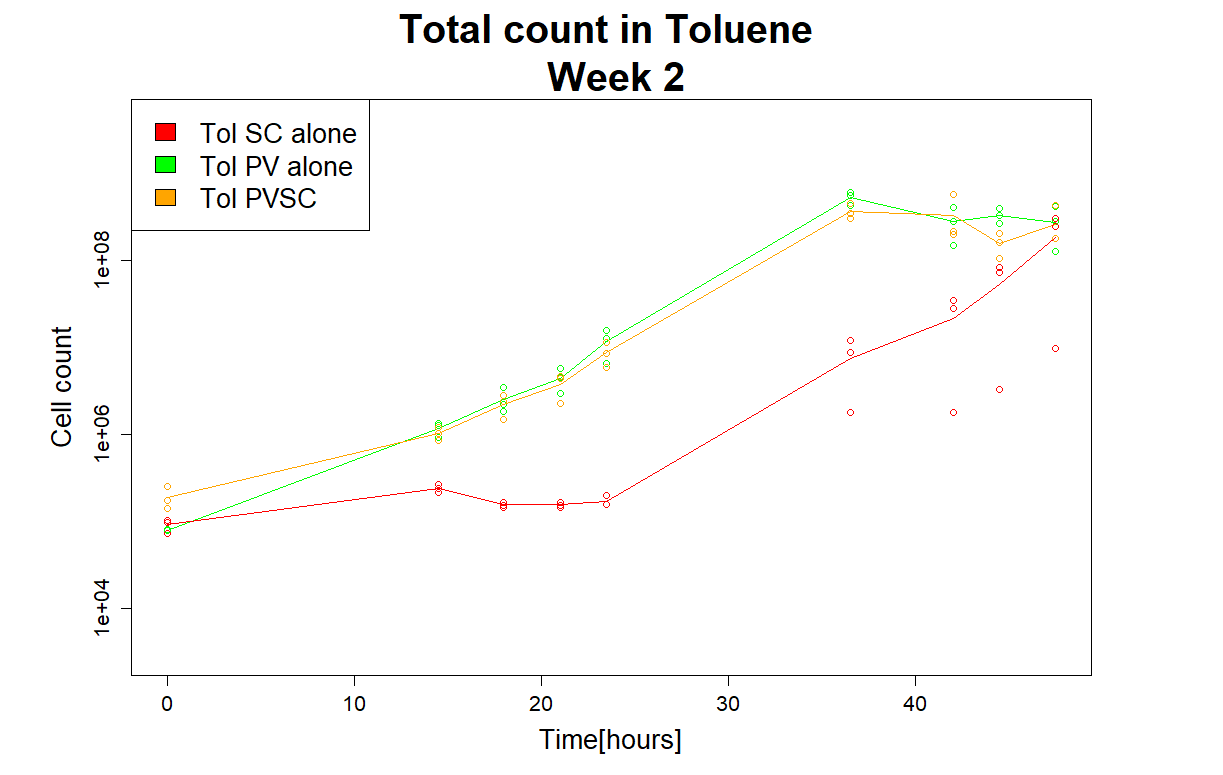
\includegraphics[width=7.71cm]{totcount_tol2.png}
			%		\phantomsubcaption
			\caption{}
			%		\caption{Growth curves of total count in toluene, Experiment 2}
			\label{totcounttol2}
		\end{subfigure}%	
		\begin{subfigure}{.47\textheight}
			\centering
			\vspace{-0cm}	
			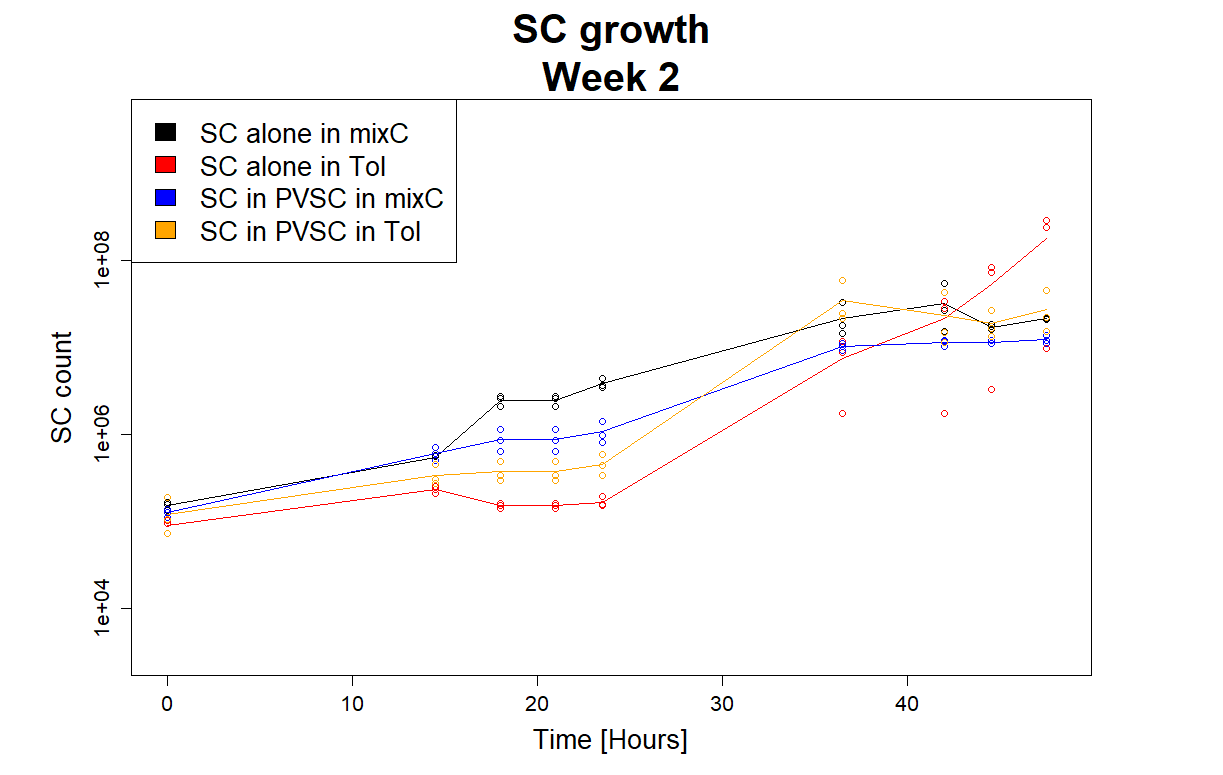
\includegraphics[width=7.71cm]{SCgrowth2.png}
			%		\phantomsubcaption
			\caption{}
			%		\caption{SC Growth curves, Experiment 2}
			\label{SCgrowth2}
		\end{subfigure}%
		\begin{subfigure}{.47\textheight}
			\centering
			\vspace{-0cm}
			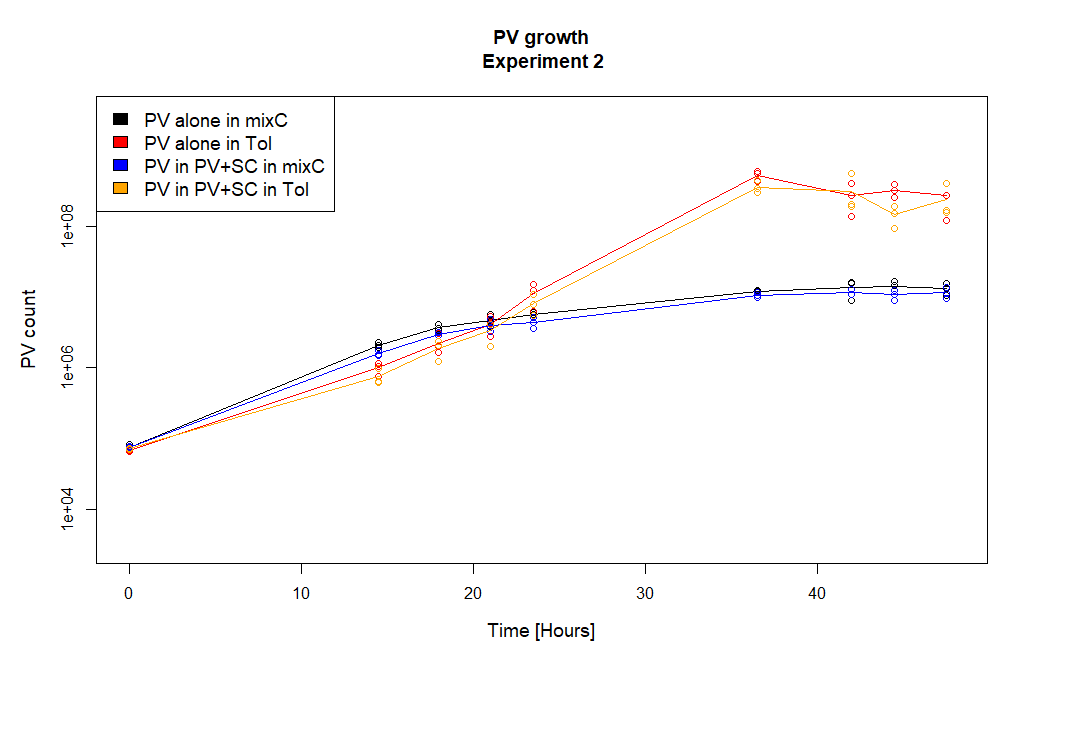
\includegraphics[width=7.71cm]{PVgrowth2.png}
			%		\phantomsubcaption
			\caption{}
			%		\caption{PP Growth curves, Experiment 2}
			\label{PVgrowth2}
		\end{subfigure}
		
		\caption{ Growth curves of: Fig. \ref{totcountmixC1}, Total count in Mixed Carbon, Week 1; Fig. \ref{totcounttol1}, Total count of cells in toluene, Week 2; Fig. \ref{SCgrowth1}, SC growth in different substrates, Week 1; Fig. \ref{PPgrowth1}, SC growth in different substrates, Week 1; Fig. \ref{totcountmixC2}, Total count in Mixed Carbon, Week 2; Fig. \ref{totcounttol2}, Total count of cells in toluene, Week 2; Fig. \ref{SCgrowth2}, SC growth in different substrates, Week 2; Fig. \ref{PVgrowth2}, SC growth in different substrates, Week 2.}
		
		
	\end{figure}
\end{landscape}

\end{document}
